% Options for packages loaded elsewhere
\PassOptionsToPackage{unicode}{hyperref}
\PassOptionsToPackage{hyphens}{url}
\PassOptionsToPackage{dvipsnames,svgnames,x11names}{xcolor}
%
\documentclass[
  letterpaper,
  DIV=11,
  numbers=noendperiod]{scrartcl}

\usepackage{amsmath,amssymb}
\usepackage{iftex}
\ifPDFTeX
  \usepackage[T1]{fontenc}
  \usepackage[utf8]{inputenc}
  \usepackage{textcomp} % provide euro and other symbols
\else % if luatex or xetex
  \usepackage{unicode-math}
  \defaultfontfeatures{Scale=MatchLowercase}
  \defaultfontfeatures[\rmfamily]{Ligatures=TeX,Scale=1}
\fi
\usepackage{lmodern}
\ifPDFTeX\else  
    % xetex/luatex font selection
\fi
% Use upquote if available, for straight quotes in verbatim environments
\IfFileExists{upquote.sty}{\usepackage{upquote}}{}
\IfFileExists{microtype.sty}{% use microtype if available
  \usepackage[]{microtype}
  \UseMicrotypeSet[protrusion]{basicmath} % disable protrusion for tt fonts
}{}
\makeatletter
\@ifundefined{KOMAClassName}{% if non-KOMA class
  \IfFileExists{parskip.sty}{%
    \usepackage{parskip}
  }{% else
    \setlength{\parindent}{0pt}
    \setlength{\parskip}{6pt plus 2pt minus 1pt}}
}{% if KOMA class
  \KOMAoptions{parskip=half}}
\makeatother
\usepackage{xcolor}
\setlength{\emergencystretch}{3em} % prevent overfull lines
\setcounter{secnumdepth}{5}
% Make \paragraph and \subparagraph free-standing
\ifx\paragraph\undefined\else
  \let\oldparagraph\paragraph
  \renewcommand{\paragraph}[1]{\oldparagraph{#1}\mbox{}}
\fi
\ifx\subparagraph\undefined\else
  \let\oldsubparagraph\subparagraph
  \renewcommand{\subparagraph}[1]{\oldsubparagraph{#1}\mbox{}}
\fi


\providecommand{\tightlist}{%
  \setlength{\itemsep}{0pt}\setlength{\parskip}{0pt}}\usepackage{longtable,booktabs,array}
\usepackage{calc} % for calculating minipage widths
% Correct order of tables after \paragraph or \subparagraph
\usepackage{etoolbox}
\makeatletter
\patchcmd\longtable{\par}{\if@noskipsec\mbox{}\fi\par}{}{}
\makeatother
% Allow footnotes in longtable head/foot
\IfFileExists{footnotehyper.sty}{\usepackage{footnotehyper}}{\usepackage{footnote}}
\makesavenoteenv{longtable}
\usepackage{graphicx}
\makeatletter
\def\maxwidth{\ifdim\Gin@nat@width>\linewidth\linewidth\else\Gin@nat@width\fi}
\def\maxheight{\ifdim\Gin@nat@height>\textheight\textheight\else\Gin@nat@height\fi}
\makeatother
% Scale images if necessary, so that they will not overflow the page
% margins by default, and it is still possible to overwrite the defaults
% using explicit options in \includegraphics[width, height, ...]{}
\setkeys{Gin}{width=\maxwidth,height=\maxheight,keepaspectratio}
% Set default figure placement to htbp
\makeatletter
\def\fps@figure{htbp}
\makeatother
\newlength{\cslhangindent}
\setlength{\cslhangindent}{1.5em}
\newlength{\csllabelwidth}
\setlength{\csllabelwidth}{3em}
\newlength{\cslentryspacingunit} % times entry-spacing
\setlength{\cslentryspacingunit}{\parskip}
\newenvironment{CSLReferences}[2] % #1 hanging-ident, #2 entry spacing
 {% don't indent paragraphs
  \setlength{\parindent}{0pt}
  % turn on hanging indent if param 1 is 1
  \ifodd #1
  \let\oldpar\par
  \def\par{\hangindent=\cslhangindent\oldpar}
  \fi
  % set entry spacing
  \setlength{\parskip}{#2\cslentryspacingunit}
 }%
 {}
\usepackage{calc}
\newcommand{\CSLBlock}[1]{#1\hfill\break}
\newcommand{\CSLLeftMargin}[1]{\parbox[t]{\csllabelwidth}{#1}}
\newcommand{\CSLRightInline}[1]{\parbox[t]{\linewidth - \csllabelwidth}{#1}\break}
\newcommand{\CSLIndent}[1]{\hspace{\cslhangindent}#1}

\usepackage{booktabs}
\usepackage{longtable}
\usepackage{array}
\usepackage{multirow}
\usepackage{wrapfig}
\usepackage{float}
\usepackage{colortbl}
\usepackage{pdflscape}
\usepackage{tabu}
\usepackage{threeparttable}
\usepackage{threeparttablex}
\usepackage[normalem]{ulem}
\usepackage{makecell}
\usepackage{xcolor}
\usepackage{siunitx}

  \newcolumntype{d}{S[
    input-open-uncertainty=,
    input-close-uncertainty=,
    parse-numbers = false,
    table-align-text-pre=false,
    table-align-text-post=false
  ]}
  
\KOMAoption{captions}{tableheading}
\usepackage{pdfpages}
\usepackage[margin=1in]{geometry}
\makeatletter
\makeatother
\makeatletter
\makeatother
\makeatletter
\@ifpackageloaded{caption}{}{\usepackage{caption}}
\AtBeginDocument{%
\ifdefined\contentsname
  \renewcommand*\contentsname{Table of contents}
\else
  \newcommand\contentsname{Table of contents}
\fi
\ifdefined\listfigurename
  \renewcommand*\listfigurename{List of Figures}
\else
  \newcommand\listfigurename{List of Figures}
\fi
\ifdefined\listtablename
  \renewcommand*\listtablename{List of Tables}
\else
  \newcommand\listtablename{List of Tables}
\fi
\ifdefined\figurename
  \renewcommand*\figurename{Figure}
\else
  \newcommand\figurename{Figure}
\fi
\ifdefined\tablename
  \renewcommand*\tablename{Table}
\else
  \newcommand\tablename{Table}
\fi
}
\@ifpackageloaded{float}{}{\usepackage{float}}
\floatstyle{ruled}
\@ifundefined{c@chapter}{\newfloat{codelisting}{h}{lop}}{\newfloat{codelisting}{h}{lop}[chapter]}
\floatname{codelisting}{Listing}
\newcommand*\listoflistings{\listof{codelisting}{List of Listings}}
\makeatother
\makeatletter
\@ifpackageloaded{caption}{}{\usepackage{caption}}
\@ifpackageloaded{subcaption}{}{\usepackage{subcaption}}
\makeatother
\makeatletter
\@ifpackageloaded{tcolorbox}{}{\usepackage[skins,breakable]{tcolorbox}}
\makeatother
\makeatletter
\@ifundefined{shadecolor}{\definecolor{shadecolor}{rgb}{.97, .97, .97}}
\makeatother
\makeatletter
\makeatother
\makeatletter
\makeatother
\ifLuaTeX
  \usepackage{selnolig}  % disable illegal ligatures
\fi
\IfFileExists{bookmark.sty}{\usepackage{bookmark}}{\usepackage{hyperref}}
\IfFileExists{xurl.sty}{\usepackage{xurl}}{} % add URL line breaks if available
\urlstyle{same} % disable monospaced font for URLs
\hypersetup{
  pdftitle={Forecasting the 2024 U.S. Presidential Election: An Analysis for Battleground States},
  pdfauthor={Shamayla Durrin; Denise Chang; Krishna Kumar},
  colorlinks=true,
  linkcolor={blue},
  filecolor={Maroon},
  citecolor={Blue},
  urlcolor={Blue},
  pdfcreator={LaTeX via pandoc}}

\title{Forecasting the 2024 U.S. Presidential Election: An Analysis for
Battleground States\thanks{Code and data are available at:
\url{https://github.com/krishnak30/US_elections}.}}
\usepackage{etoolbox}
\makeatletter
\providecommand{\subtitle}[1]{% add subtitle to \maketitle
  \apptocmd{\@title}{\par {\large #1 \par}}{}{}
}
\makeatother
\subtitle{Trump Favored Nationally, While Harris Leads in 4 of 7
Battleground States}
\author{Shamayla Durrin \and Denise Chang \and Krishna Kumar}
\date{November 1, 2024}

\begin{document}
\maketitle
\begin{abstract}
This study employs a polls-of-polls approach to predict support for
Kamala Harris and Donald Trump in the 2024 U.S. Presidential Election,
with a focus on key battleground states to forecast the likely winner of
the electoral college. By aggregating multiple polls and applying a
weighted linear regression model with predictors like pollster
reliability, sample size, state, and recency, we estimate a higher
national support for Trump relative to Harris. Our analysis also reveals
a close competition in battleground states, with Trump holding a narrow
lead in Arizona, Georgia, and North Carolina, while Harris leads in
Michigan, Nevada, Pennsylvania, and Wisconsin. These findings underscore
the value of aggregating polls over relying on individual surveys,
offering a more comprehensive and robust forecast of electoral outcomes.
\end{abstract}
\ifdefined\Shaded\renewenvironment{Shaded}{\begin{tcolorbox}[enhanced, boxrule=0pt, interior hidden, borderline west={3pt}{0pt}{shadecolor}, breakable, sharp corners, frame hidden]}{\end{tcolorbox}}\fi

\vspace{0.7cm}

\hypertarget{introduction}{%
\section{Introduction}\label{introduction}}

While individual polls provide snapshots of public opinion, they are
often subject to biases and methodological differences. In this paper,
we aim to forecast voter support for Kamala Harris and Donald Trump by
aggregating data from multiple polling sources, reducing individual poll
biases, and improving overall prediction accuracy. Our analysis focuses
on estimating the levels of support for each candidate not only
nationally but also in key swing states that are likely to be decisive
in determining the electoral college outcome.

The estimand of this study is the level of voter support for each
candidate, Kamala Harris and Donald Trump, as reported across multiple
polls.To estimate this, we developed a regression model incorporating
variables such as pollster, sample size, state, and recency of the poll,
with an emphasis on accurately capturing state-level dynamics. Our
findings indicate that, on a national level, support between Kamala
Harris and Donald Trump is closely balanced. Harris's estimated national
support stands close to 48\%, while Trump's support is slightly higher,
around 49\%. We found that Trump holds a marginal lead in battleground
states like Arizona and Georgia, with a support margin slightly above
1\%. In contrast, Harris shows narrow leads in Michigan, Nevada,
Pennsylvania, and Wisconsin, with her support margin in Wisconsin
reaching over 2\%, making it her strongest battleground. North Carolina
emerges as one of the tightest races, with Trump leading by only 0.26\%,
underscoring the competitive nature of these regions.

This paper contributes to the field of election forecasting by
emphasizing the importance of poll quality and recency in prediction
models. By focusing on battleground states where the support margins are
particularly close, our approach highlights the areas where campaign
strategies and voter turnout efforts may have the greatest impact. This
could provides insights for political strategists, media analysts, and
the general public by offering a nuanced view of the electoral
landscape.

This paper is organized as follows: In \ref{sec-data}, we clean the
data, explore summary statistics, plot distributions of key variables,
and examine relationships between variables. In \ref{sec-model}, we
discuss our forecasting approach, model selection, justification for the
chosen model, and the mechanism of deriving poll weights based on
pollster reliability, ultimately presenting our predictions. Finally, in
\ref{sec-discussion}, we address the broader implications of our
findings, acknowledge limitations, and suggest directions for future
work.

\vspace{0.7cm}

\hypertarget{sec-data}{%
\section{Data}\label{sec-data}}

\vspace{0.7cm}

\hypertarget{data-cleaning}{%
\subsection{Data Cleaning}\label{data-cleaning}}

The raw data for this project, sourced from FiveThirtyEight,
(FiveThirtyEight 2024) underwent a series of cleaning steps to prepare
it for analysis. Initially, duplicate rows were removed to ensure that
only unique observations remained, facilitated by the \texttt{janitor}
package (Firke 2023). A new binary variable, `national', was created to
indicate whether a poll was conducted at the national or state level.
Missing values in the `state' column were replaced with ``Not
Applicable,'' and numeric grades were evaluated to filter out
low-quality pollsters, keeping only those with a numeric grade above 1.
This cutoff was selected to retain mid to high-level pollsters for more
reliable results. These steps were performed using functions from the
\texttt{tidyverse} package (Wickham et al. 2019). Dates were also
standardized and converted into a proper format for analysis using the
same package. Polls related to Kamala Harris were retained for further
analysis, and percentage support values were transformed into actual
numbers of supporters based on sample size. Additionally, pollster
counts below five were excluded to focus on more reliable data sources.
Polls regarding Kamala Harris were filtered to include only those
conducted after her official candidacy announcement on July 21, 2024,
ensuring the data reflects post-announcement public sentiment.The
cleaned dataset was saved in Parquet format for efficient storage and
retrieval, using the \texttt{arrow} package (Richardson et al. 2024).

\hypertarget{explorations-of-variables-of-interest}{%
\subsection{Explorations of Variables of
Interest}\label{explorations-of-variables-of-interest}}

\hypertarget{summary-statistics-of-key-variables-and-measurement-method}{%
\subsubsection{Summary Statistics of Key Variables and Measurement
Method}\label{summary-statistics-of-key-variables-and-measurement-method}}

\vspace{0.7cm}

For the purposes this analysis, a subset of variables was selected from
the raw data set. Two additional variables, `national' and `state', were
created using the existing `state' and `end date' variable. A short
description of each variable of interest and their respective
measurement methods is given below.

\begin{itemize}
\item
  \emph{Pollster}: The name of the polling organization conducting the
  poll (e.g., YouGov, RMG Research). This variable helps adjust for
  poll-specific biases. Every pollster that publicly published a
  scientific poll about the 2024 U.S. Presidential Election is included
  in the data set. The value measured for this variable is the name that
  appears in the scientific poll (Morris 2024b).
\item
  \emph{Numeric Grade}: A numeric rating given to the pollster,
  representing the accuracy and methodological transparency of the
  organization (e.g., 3.0), with higher grades indicating more reliable
  pollsters. The value of this variable is calculated by the 538 team.
  All national and state-level polls that were conducted in 1998 or
  later are considered to determine and to assign a numeric grade to
  each pollster (Morris 2024a).
\item
  \emph{Pollscore}: A score that reflects the reliability of each
  pollster, capturing their historical accuracy and biases. Negative
  values indicate better predictive accuracy, and rewards pollsters who
  are accurate and precise. This variable is calculated by aggregating
  predictive error and predictive bias together (Morris 2024a).
  Predictive error is the difference between expectations and reality
  (Renewable Energy 2012) and predictive bias is the systematic bias
  introduced in the methodology (Aguinis and Culpepper 2024).
\item
  \emph{State}: The U.S. state where the poll was conducted, allowing
  for analysis of regional differences in candidate support. The value
  measured for this variable is the primary state that appears in the
  scientific poll's methodology (Morris 2024b).
\item
  \emph{National}: A binary variable indicating whether the poll is
  national (1 for national polls, 0 for state polls).
\item
  \emph{End Date}: The date the poll ended, reflecting the currency of
  the data. This variable is taken from the publication, and is the last
  date for which the survey was active (Morris 2024b).
\item
  \emph{Sample Size}: The total number of respondents in the poll. This
  is measure by the number of completed surveys (Morris 2024b).
\item
  \emph{Candidate Name}: The name of the candidate being polled (e.g.,
  Kamala Harris or Donald Trump), identifying the focus of each poll
  result.
\item
  \emph{Pct (Percentage)}: The percentage of respondents in the poll who
  support the specified candidate.
\item
  \emph{Recency}: This variable measures how recent each poll is. This
  variable is calculated by subtracting the end date of the poll from
  the end date of the most recent poll.
\end{itemize}

\newpage

\hypertarget{tbl-sumstat}{}
\begin{table}
\caption{\label{tbl-sumstat}Summary Statistics of Numerical Variable }\tabularnewline

\centering
\begin{tabular}[t]{lrrrrrrr}
\toprule
  & Unique (\#) & Missing (\%) & Mean & SD & Min & Median & Max\\
\midrule
numeric\_grade & 21 & 0 & \num{2.2} & \num{0.6} & \num{1.0} & \num{2.1} & \num{3.0}\\
pollscore & 21 & 0 & \num{-0.5} & \num{0.6} & \num{-1.5} & \num{-0.4} & \num{1.7}\\
sample\_size & 594 & 0 & \num{1908.8} & \num{2602.0} & \num{147.0} & \num{999.0} & \num{20762.0}\\
pct & 216 & 0 & \num{46.9} & \num{4.0} & \num{25.0} & \num{47.0} & \num{70.0}\\
recency & 91 & 0 & \num{43.6} & \num{25.9} & \num{0.0} & \num{41.0} & \num{90.0}\\
\bottomrule
\end{tabular}
\end{table}

\vspace{0.7cm}

Table~\ref{tbl-sumstat} shows that the average poll in our dataset has a
numeric grade of 2.2. This suggests most polls are of moderate to high
quality in terms of reliability. The mean pollscore of -0.5 suggests
these polls are relatively accurate, as negative values imply reduced
bias. Additionally, the large average sample size of 1908 respondents
across polls provides a stable basis for our model, reducing variability
and ensuring reliable predictions for candidate support.

\newpage

\hypertarget{variation-of-poll-quality-and-support-for-candiates-by-pollster}{%
\subsubsection{Variation of Poll Quality and Support for Candiates by
Pollster}\label{variation-of-poll-quality-and-support-for-candiates-by-pollster}}

\vspace{0.7cm}

\hypertarget{tbl-topster}{}
\begin{longtable}[]{@{}
  >{\raggedright\arraybackslash}p{(\columnwidth - 6\tabcolsep) * \real{0.3867}}
  >{\raggedleft\arraybackslash}p{(\columnwidth - 6\tabcolsep) * \real{0.0800}}
  >{\raggedleft\arraybackslash}p{(\columnwidth - 6\tabcolsep) * \real{0.2400}}
  >{\raggedleft\arraybackslash}p{(\columnwidth - 6\tabcolsep) * \real{0.2933}}@{}}
\caption{\label{tbl-topster}Top 5 most frequent pollsters, with count of
polls, average pollscore (lower scores indicate less bias), and average
numeric grade (higher values indicate greater
reliability).}\tabularnewline
\toprule\noalign{}
\begin{minipage}[b]{\linewidth}\raggedright
Pollster
\end{minipage} & \begin{minipage}[b]{\linewidth}\raggedleft
Count
\end{minipage} & \begin{minipage}[b]{\linewidth}\raggedleft
Average Pollscore
\end{minipage} & \begin{minipage}[b]{\linewidth}\raggedleft
Average Numeric Grade
\end{minipage} \\
\midrule\noalign{}
\endfirsthead
\toprule\noalign{}
\begin{minipage}[b]{\linewidth}\raggedright
Pollster
\end{minipage} & \begin{minipage}[b]{\linewidth}\raggedleft
Count
\end{minipage} & \begin{minipage}[b]{\linewidth}\raggedleft
Average Pollscore
\end{minipage} & \begin{minipage}[b]{\linewidth}\raggedleft
Average Numeric Grade
\end{minipage} \\
\midrule\noalign{}
\endhead
\bottomrule\noalign{}
\endlastfoot
Morning Consult & 470 & -0.3 & 1.9 \\
Siena/NYT & 188 & -1.5 & 3.0 \\
Redfield \& Wilton Strategies & 176 & 0.4 & 1.8 \\
Emerson & 116 & -1.1 & 2.9 \\
YouGov & 113 & -1.1 & 3.0 \\
\end{longtable}

Table~\ref{tbl-topster} displays the top 5 most frequent pollsters in
the dataset, with each pollster's total poll count, average pollscore
(measuring reliability and historical accuracy), and average numeric
grade (indicating overall quality). We observe that the most frequent
pollster, Morning Consult, has a moderate pollscore and a slightly
above-average numeric grade, indicating it provides fairly reliable
data. However, there is variability in pollscore and numeric grade
across the top pollsters, reflecting differences in quality and
potential biases among them, which the model needs to adjust for to
achieve accurate predictions.

\begin{figure}

{\centering 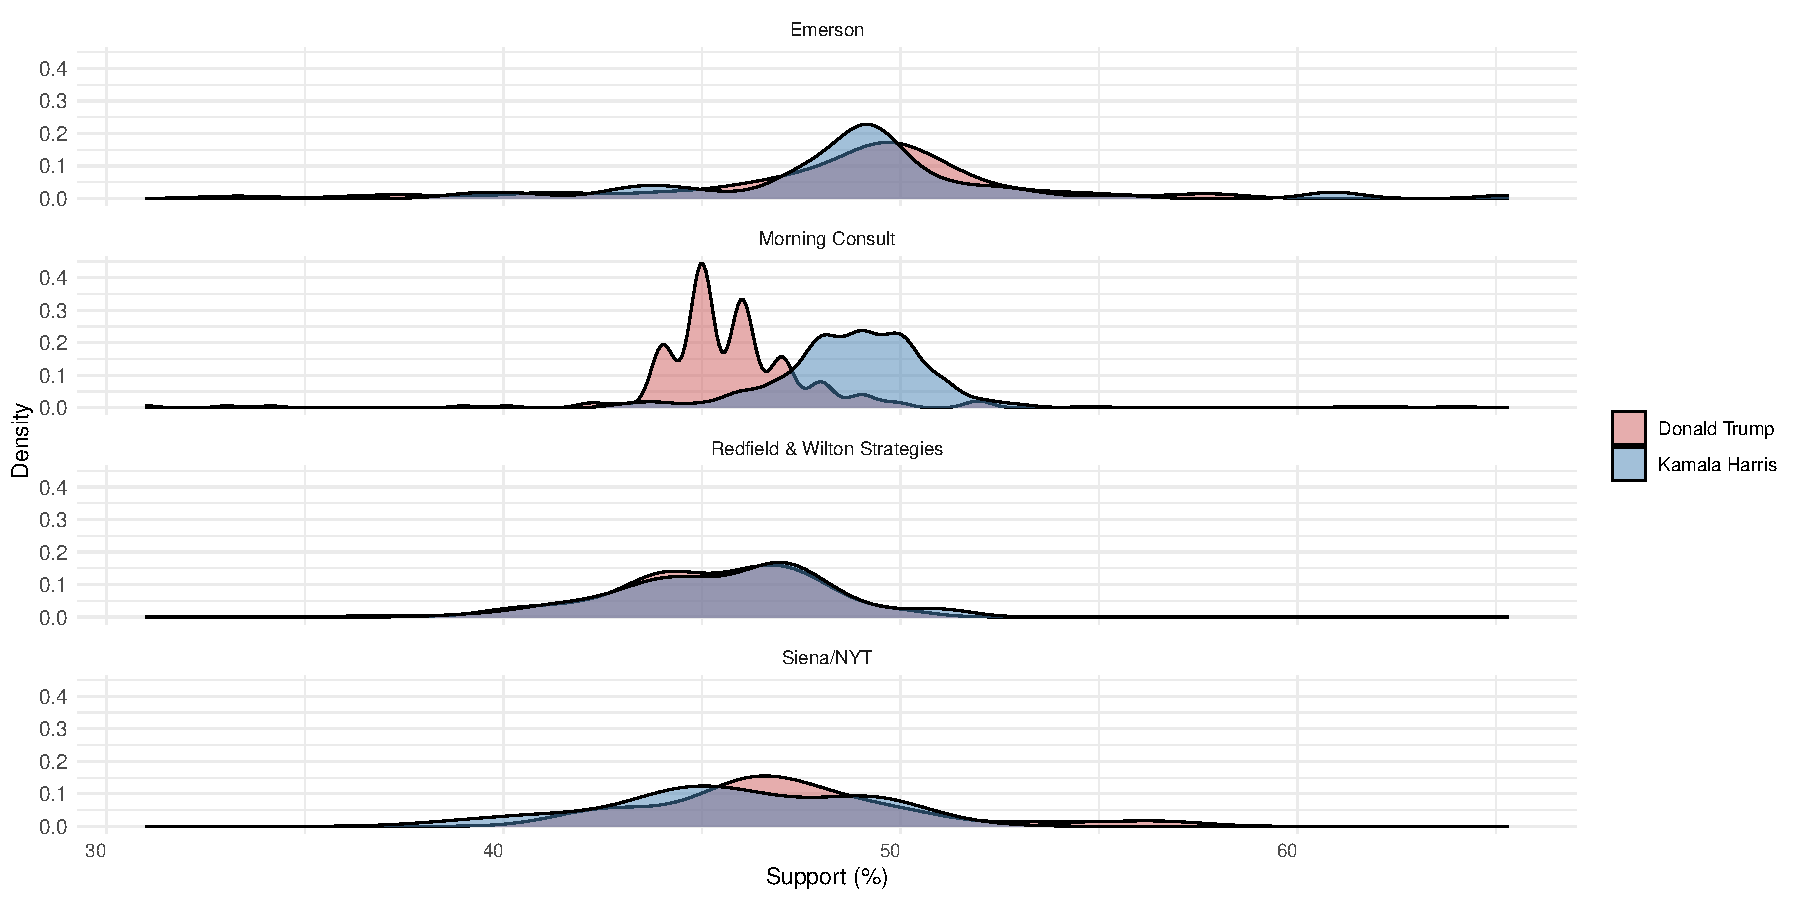
\includegraphics{paper_files/figure-pdf/fig-ster-1.pdf}

}

\caption{\label{fig-ster}Support distribution for Kamala Harris and
Donald Trump by major pollsters, highlighting variability in reported
support across organizations and the value of aggregating multiple polls
for balanced insights.}

\end{figure}

Figure~\ref{fig-ster} shows the distribution of support for Kamala
Harris and Donald Trump by pollster, highlighting variability across
different polling organizations. Morning Consult, for example,
demonstrates a wide range in reported support, with more spread in
Trump's support. In contrast, Siena/NYT shows less variation, with
Harris consistently leading. This variability across pollsters
emphasizes the importance of aggregating multiple polls to account for
organization-specific biases and ensure a more balanced view of
candidate support.

\hypertarget{sample-size-of-polls}{%
\subsubsection{Sample Size of Polls}\label{sample-size-of-polls}}

\vspace{0.7cm}

\begin{figure}

{\centering 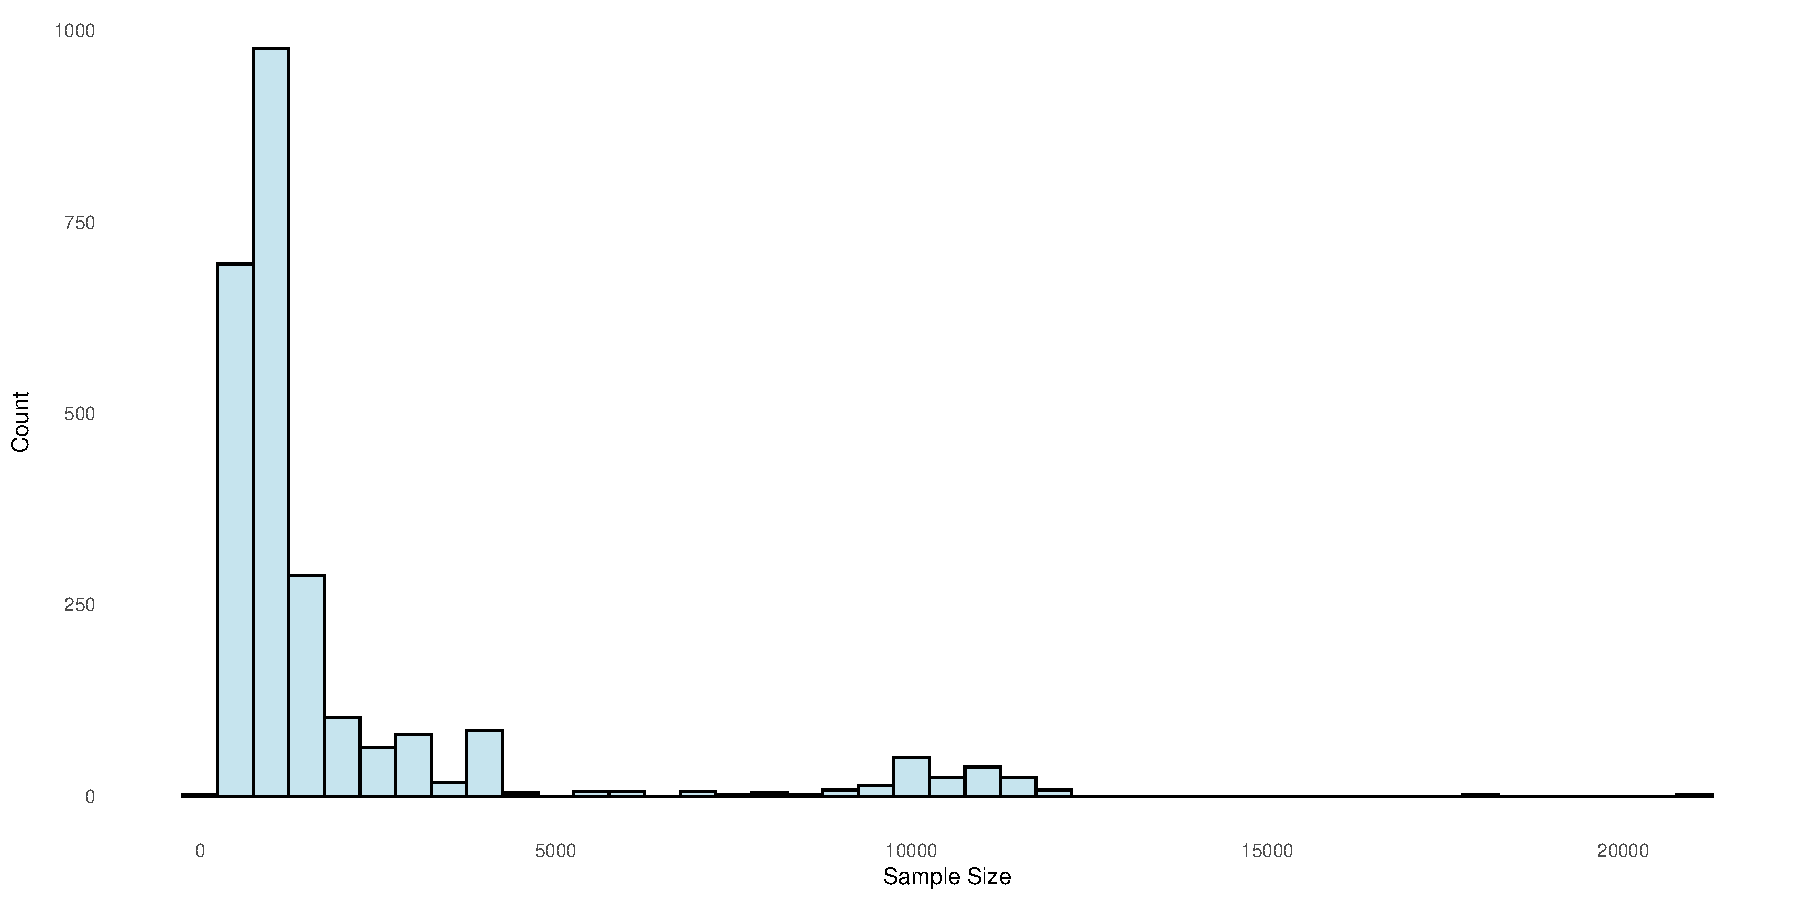
\includegraphics{paper_files/figure-pdf/fig-ss-1.pdf}

}

\caption{\label{fig-ss}Distribution of Sample Sizes Across Polls:
Majority of polls have sample sizes under 5,000, with a few outliers at
larger sizes.}

\end{figure}

Figure~\ref{fig-ss} shows a clear right-skewed distribution. Most of the
sample sizes are clustered between 0 and 3000 respondents, with a sharp
peak around 1000-1500 respondents. This indicates that the majority of
polls have smaller sample sizes. As sample size increases, the frequency
significantly drops, with very few polls conducted with sample sizes
larger than 5000, though there are a few outliers with sizes approaching
10,000 or more. This wide range in sample sizes can affect the precision
of estimates across different polls.

\hypertarget{distribution-of-numeric-grade-and-pollscore-of-polls}{%
\subsubsection{Distribution of Numeric Grade and Pollscore of
Polls}\label{distribution-of-numeric-grade-and-pollscore-of-polls}}

\begin{figure}

{\centering 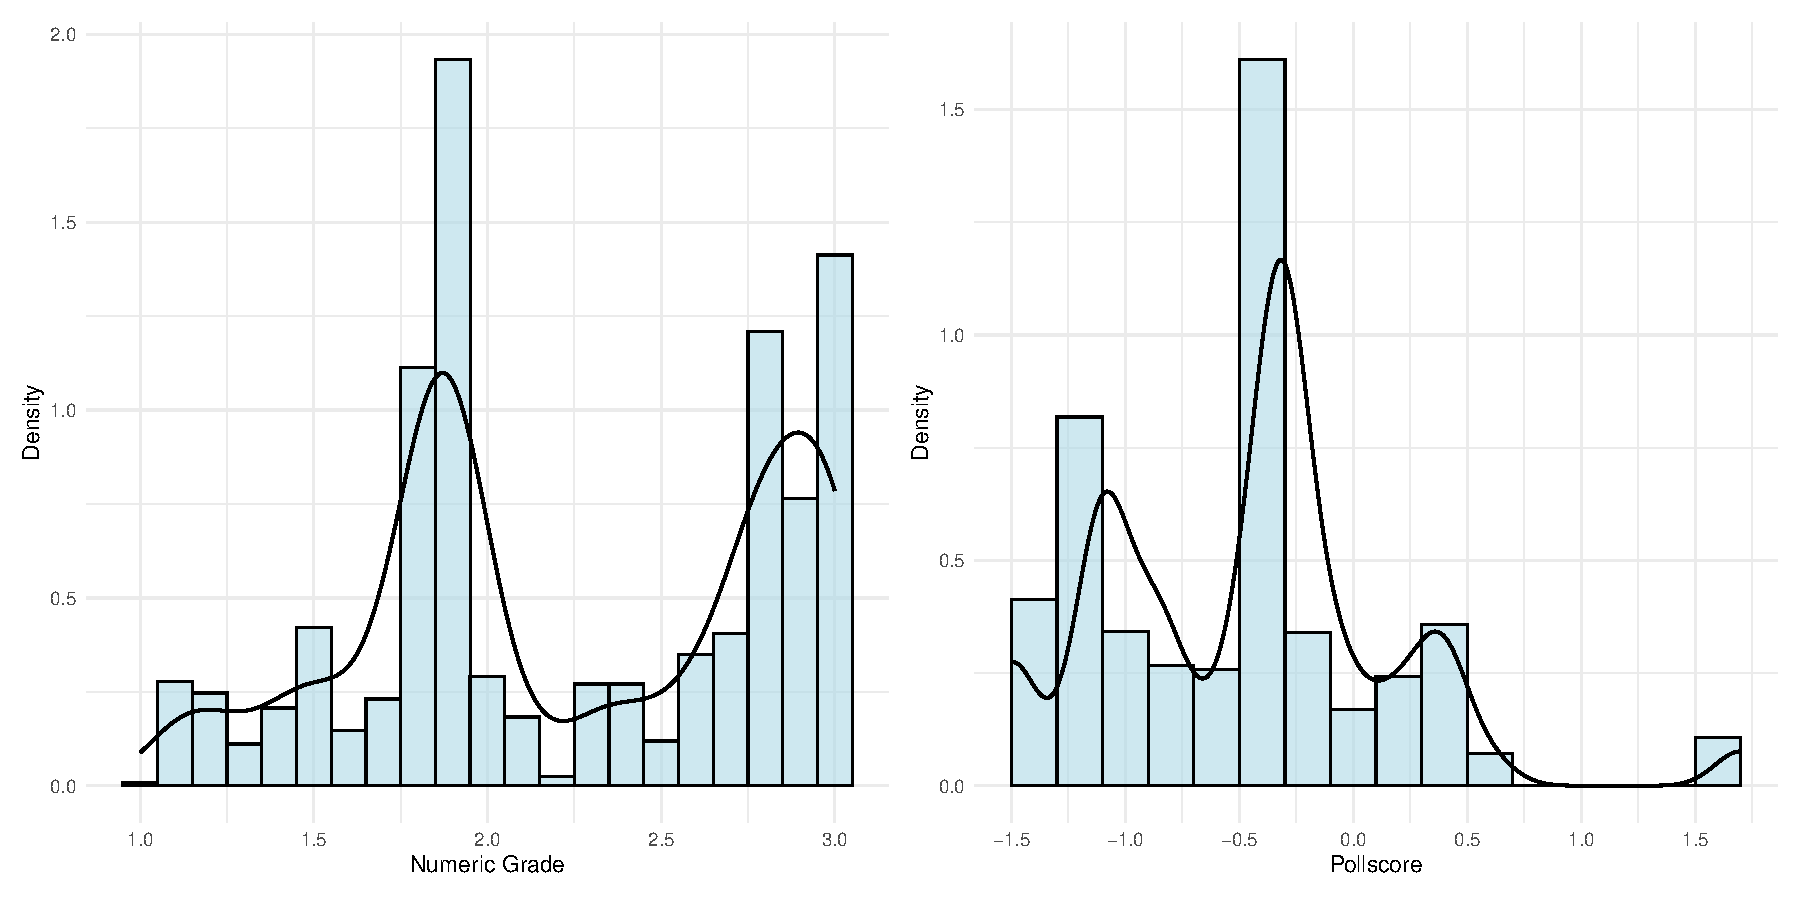
\includegraphics{paper_files/figure-pdf/fig-reli-1.pdf}

}

\caption{\label{fig-reli}Distribution of Numeric Grade and Pollscore
among polling organizations, highlighting variability in pollster
reliability and potential bias across polls.}

\end{figure}

Figure~\ref{fig-reli} shows the distribution of Numeric Grade (left) and
Pollscore (right) across polling organizations. The Numeric Grade
distribution shows that most pollsters are rated between 1.5 and 3, with
peaks around 2.0 and 2.5, indicating a concentration of pollsters with
moderate to high reliability scores. In contrast, the Pollscore
distribution, where lower values indicate higher reliability, shows a
range primarily between -1.5 and 0, with a notable peak around -0.5.
This suggests that while many polls demonstrate relatively low bias,
there is still variability in reliability across organizations. The
distinction between these two metrics emphasizes the need to consider
both quality (Numeric Grade) and potential systematic bias (Pollscore)
when weighting polls in the model.

\vspace{0.7cm}

\hypertarget{distribution-of-polls-by-poll-type-and-candidate}{%
\subsubsection{Distribution of Polls by Poll Type and
Candidate}\label{distribution-of-polls-by-poll-type-and-candidate}}

Figure~\ref{fig-pie} illustrates the distribution of polls between
candidates and poll types. The left chart shows that the majority of
polls are conducted at the state level, with a smaller portion being
national. The right chart shows that polling is almost evenly split
between Kamala Harris and Donald Trump. This distribution underscores
the model's balanced approach to capturing state-level nuances as well
as broader national trends, providing a comprehensive view of candidate
support across different contexts

\begin{figure}

{\centering 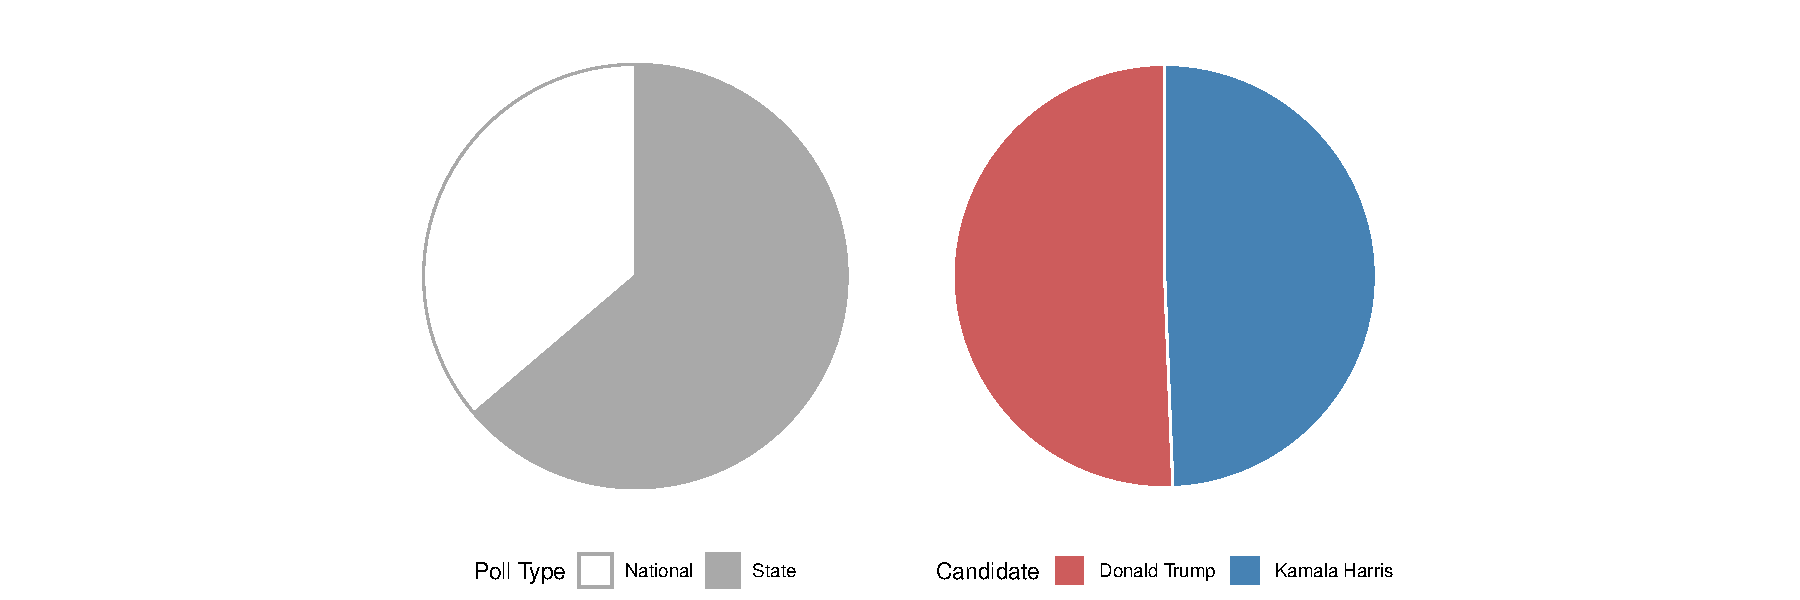
\includegraphics{paper_files/figure-pdf/fig-pie-1.pdf}

}

\caption{\label{fig-pie}Poll distribution by type (state vs.~national)
and candidate (Trump vs.~Harris), showing a majority of state polls and
near-equal coverage for each candidate.}

\end{figure}

\newpage

\hypertarget{support-trend-for-candidates}{%
\subsubsection{Support Trend For
Candidates}\label{support-trend-for-candidates}}

\begin{figure}

{\centering 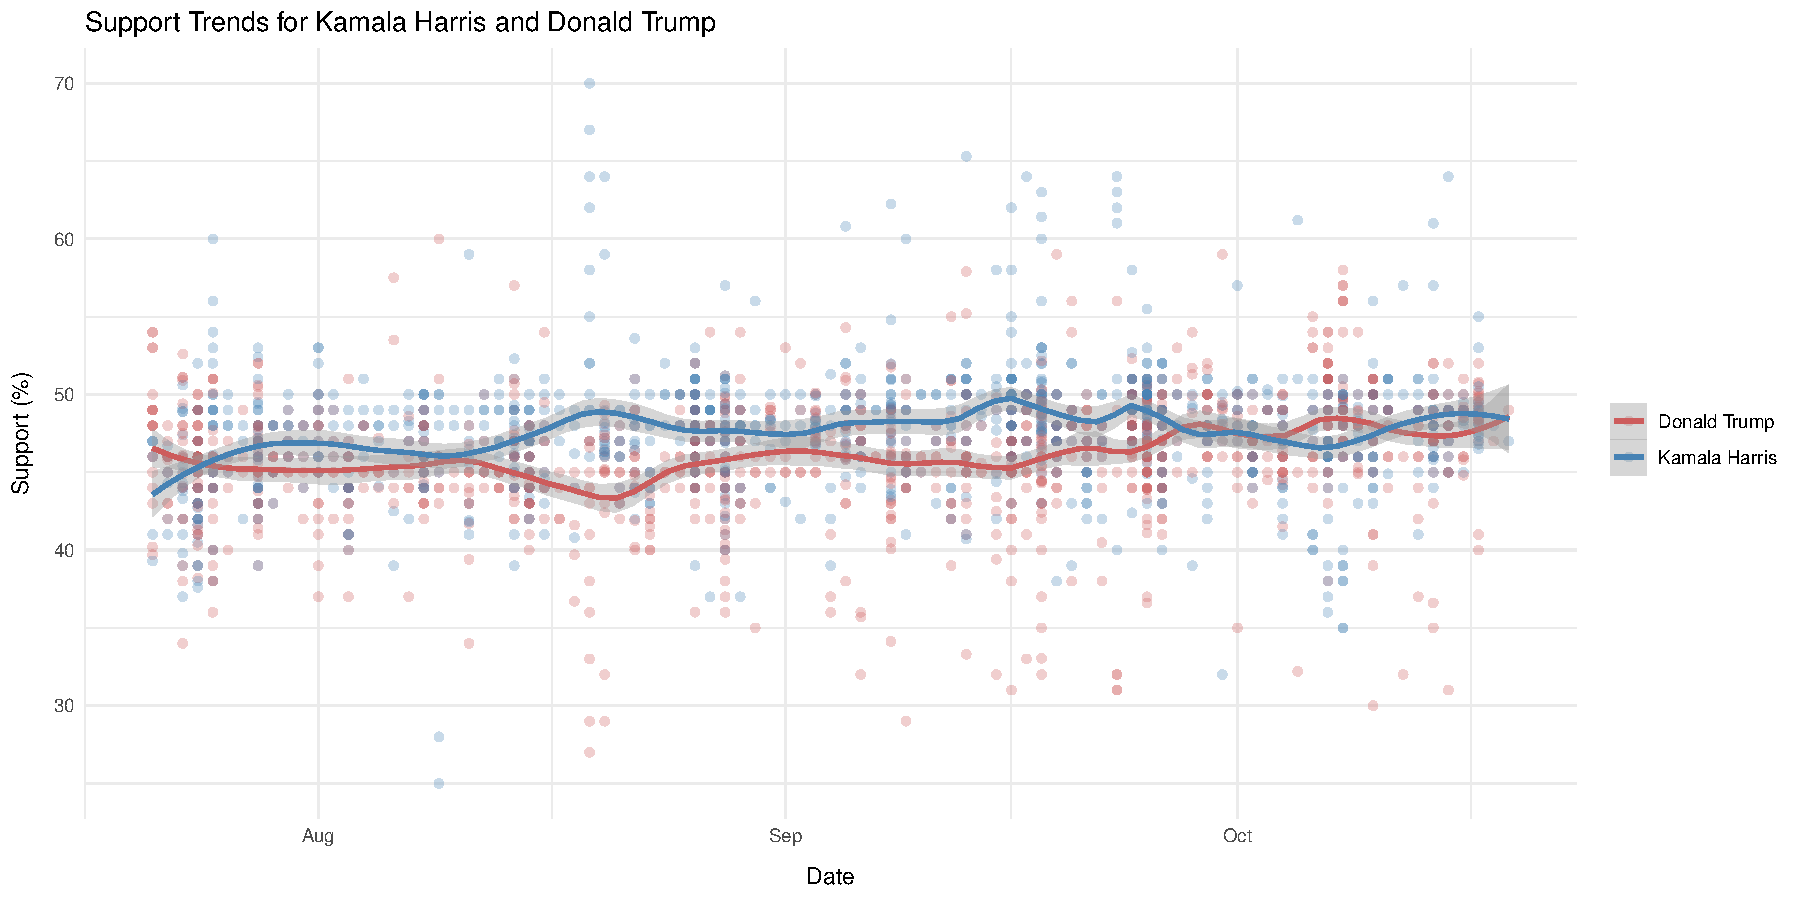
\includegraphics{paper_files/figure-pdf/fig-trend-1.pdf}

}

\caption{\label{fig-trend}Figure showing support trends for Kamala
Harris and Donald Trump over time. Trend lines indicate slight shifts in
support as the election nears, with consistent polling frequency
throughout the period.}

\end{figure}

Figure~\ref{fig-trend} shows the support trends for Kamala Harris and
Donald Trump from August to October. Each point represents a poll
result, color-coded by candidate, with the trend lines highlighting the
overall changes in support over time. Kamala Harris's support remains
relatively steady but shows slight fluctuations around mid-September,
while Donald Trump's support appears to have a small upward trend toward
October. The distribution of points is dense throughout, reflecting
consistent polling activity, though some dates show more concentrated
polling. This visualization indicates that while both candidates
maintain stable support levels, minor shifts occur as the election
approaches, underscoring the importance of tracking trends over time
rather than relying on individual polls.

\newpage

\hypertarget{relationship-between-sample-size-and-suppoert-for-candidates}{%
\subsubsection{Relationship Between Sample Size and Suppoert for
Candidates}\label{relationship-between-sample-size-and-suppoert-for-candidates}}

\begin{figure}

{\centering 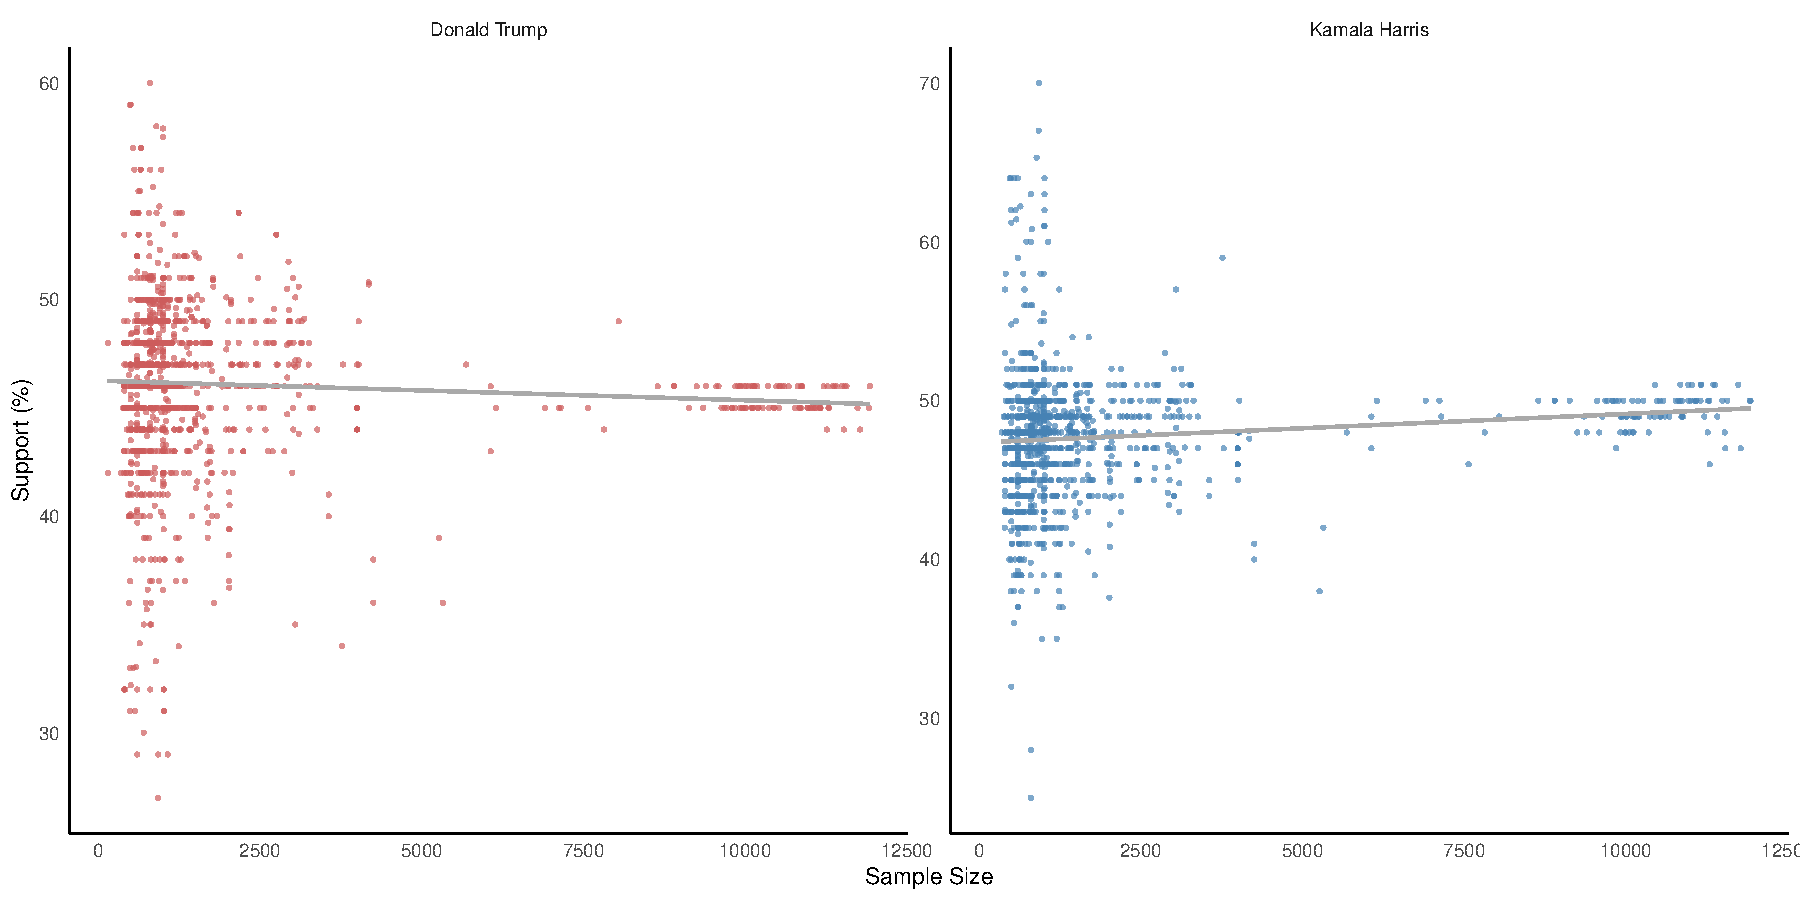
\includegraphics{paper_files/figure-pdf/fig-pct-1.pdf}

}

\caption{\label{fig-pct}Relationship between Sample Size and Support
Percentage for Donald Trump and Kamala Harris, showing slight downward
and upward trends in support with increasing sample size for Trump and
Harris, respectively.}

\end{figure}

Figure~\ref{fig-pct} shows the relationship between sample size and
support percentage for Donald Trump and Kamala Harris. For both
candidates, the majority of polls have a sample size below 2,500, but
there are some larger polls exceeding 10,000 respondents. In Trump's
chart, there's a slight downward trend, suggesting that larger sample
sizes may show marginally lower support. In contrast, Harris's chart
shows a slight upward trend with larger sample sizes, indicating a
marginal increase in support with larger poll samples. This highlights
the variability in polling support depending on the sample size,
emphasiszing the importance of including sampel size in our model.

\hypertarget{variability-of-candidate-support-across-us-states}{%
\subsubsection{Variability of Candidate support Across US
States}\label{variability-of-candidate-support-across-us-states}}

\begin{figure}

{\centering 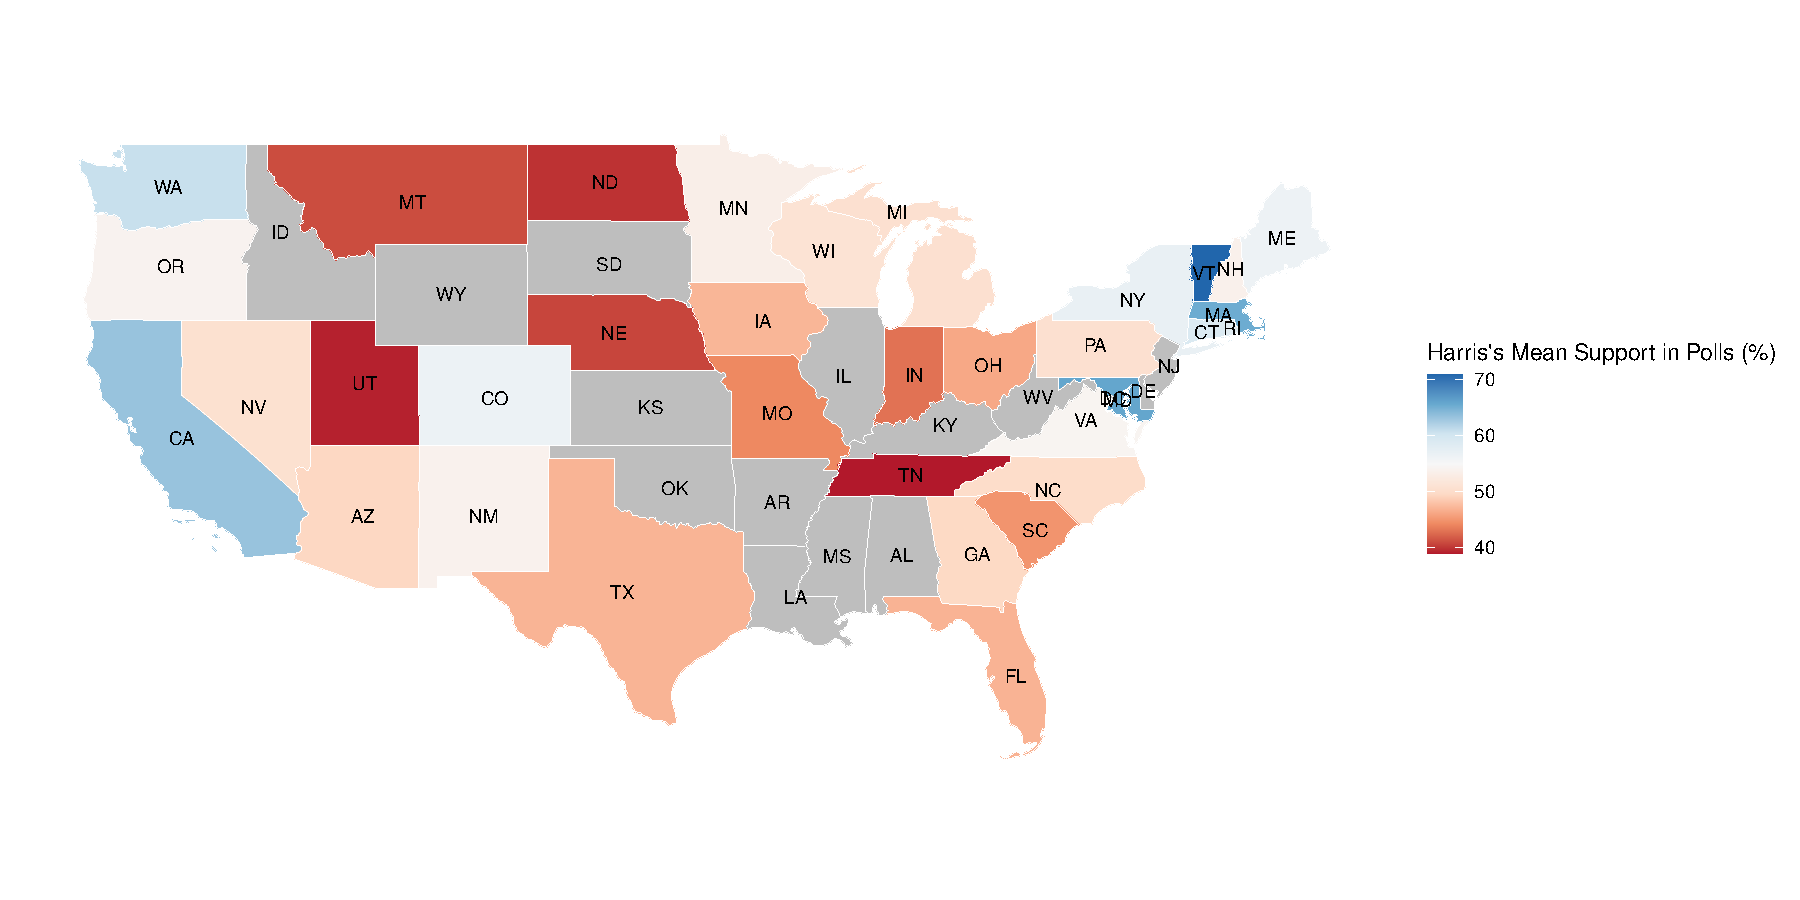
\includegraphics{paper_files/figure-pdf/fig-map1-1.pdf}

}

\caption{\label{fig-map1}Map showing the proportion of support for
Kamala Harris relative to Donald Trump across U.S. states. Blue
indicates states where Harris has higher support, while red indicates
states where Trump leads. Color intensity reflects the magnitude of
support difference, with gray indicating insufficient polling data.}

\end{figure}

Figure~\ref{fig-map1} shows the average support for Kamala Harris as a
proportion relative to both Kamala Harris and Donald Trump across the
continental U.S. states. States shaded in blue indicate a higher
proportion of support for Harris, while red shades represent stronger
support for Trump, with color intensity reflecting the support margin.
Gray-shaded states lack sufficient polling data.

In key swing states, such as Pennsylvania, Michigan, and Arizona, we
observe a balanced distribution of support, suggesting close competition
in these battleground areas. Meanwhile, traditional Democratic
strongholds, like California and New York, show a clear preference for
Harris, with deeper blue shades. Conversely, traditionally Republican
states, such as Texas and Tennessee, exhibit higher support for Trump,
with intense red shades highlighting his advantage. This visualization
emphasizes the varied regional dynamics of candidate support, with
distinct patterns in both competitive and historically partisan states.

\hypertarget{sec-model}{%
\section{Forecasting Election Outcome through Pooling
Polls}\label{sec-model}}

\hypertarget{forecasting-approach}{%
\subsection{Forecasting Approach}\label{forecasting-approach}}

The polls of polls methodology is widely used in election prediction as
it aggregates multiple polls to provide a more reliable estimate of
voter support, rather than relying on any single poll. The goal is to
reduce errors and biases present in individual polls by using a weighted
average of many different polls.

In our approach, we will employ linear modeling of voter support
percentage (pct) on pollster and other independent variables such as
sample size, poll recency, and poll scope (state vs.~national). This
will allow us to smooth out the inherent noise, biases, and variability
across different pollsters. Once we obtain the predicted values from our
model, we will weight these predictions based on the numeric grade
(quality score) of each pollster to calculate an overall national
estimate of the outcome. Additionally, we will separately compute
estimates for key battleground states, where voter behavior can be more
volatile and pivotal in deciding the final outcome of the election. This
approach helps us capture both national trends and critical state-level
dynamics.

\hypertarget{model}{%
\subsection{Model}\label{model}}

In this section, we aim to address the inherent biases and differences
present in various polling data to arrive at a robust prediction model.
The core challenge lies in selecting a model with an optimal balance
between complexity and fit, ensuring it accurately captures the dynamics
of polling data while avoiding overfitting. To this end, we carefully
evaluated different model specifications to determine the most
appropriate one for our forecasting purpose.

Given that variables like numeric grade and pollscore are perfectly
collinear with pollster, they were excluded from the regression analysis
to avoid multicollinearity issues. These variables, however, remain
integral to our weighting strategy, where they will be used to adjust
for differences in polling accuracy and reliability. Instead, we focus
on key features such as pollster, sample size, state, and recency,
gradually adding complexity to the model.

By systematically comparing model specifications that incorporate these
variables, we aim to select the model with the right balance between
predictive accuracy and generalizability, ultimately providing the best
possible forecast.

\hypertarget{model-set-up}{%
\subsection{Model Set Up}\label{model-set-up}}

We aim to model the percentage of support for Kamala Harris and Donald
Trump in each poll as a function of the pollster the sample size, the
state, and the recency of the poll.

\[
y_i = \alpha + \beta_1 \cdot \mathrm{pollster}_i + \beta_2 \cdot \mathrm{sample\_size}_i + \beta_3 \cdot \mathrm{recency}_i +  \beta_4 \cdot \mathrm{state}_i + \epsilon_i
\]

Where

\begin{itemize}
\item
  \(y_i\) is the percentage of support for candidate in poll i,
\item
  \(α\) is the intercept,
\item
  \(β_1\) captures the effect of the polling organization,
\item
  \(β_2\) captures the effect of the sample size,
\item
  \(β_3\) captures the effect of recency (how recent the poll is),
\item
  \(β_4\) capture the effects of the different states
\item
  \(\epsilon_i\) represents the error term, assumed to follow a normal
  distribution with mean 0.
\end{itemize}

\hypertarget{model-justification}{%
\subsection{Model Justification}\label{model-justification}}

\begin{figure}

{\centering 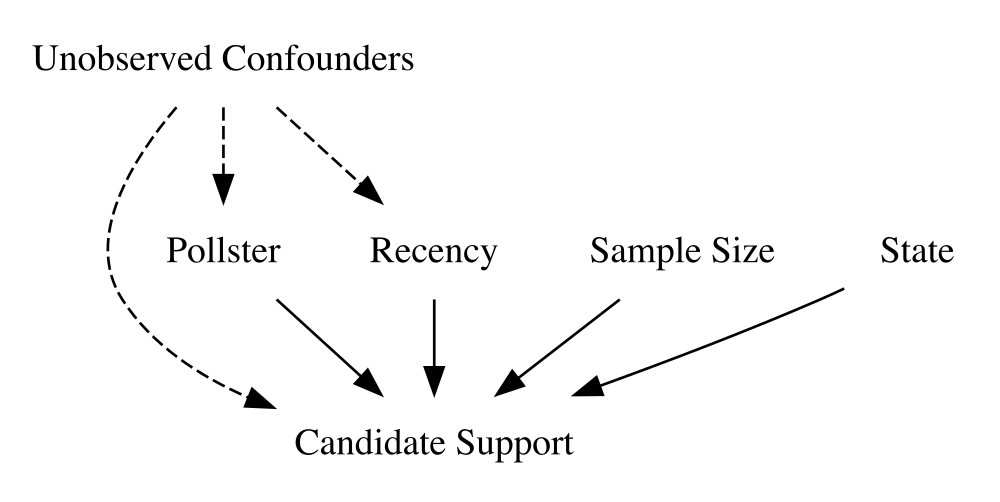
\includegraphics{../other/graphs/polls_of_polls_dag.png}

}

\caption{\label{fig-causal-model}Directed Acyclic Graph illustrating
factors influencing candidate support, with poll attributes (Pollster,
Sample Size, State, Recency) as direct contributors and unobserved
confounders representing potential biases in polling results.}

\end{figure}

In our model, we aim to smooth out discrepancies and biases across
various polling organizations using a polls-of-polls approach. Given the
potential for individual pollsters to introduce systematic
differences---due to variations in sampling methods, question phrasing,
and historical leanings---our model includes a pollster variable to
adjust for these organization-specific biases. This allows us to capture
an aggregated view of public support that is less susceptible to the
idiosyncrasies of any single poll. Furthermore, we incorporate sample
size as a predictor, as polls with larger samples tend to yield more
stable and reliable results, reducing random fluctuations caused by
smaller samples. The state variable accounts for regional political
differences, ensuring that the model captures varying levels of support
across geographic and demographic groups, which is crucial for
understanding the nuanced political landscape. Additionally, recency is
included to prioritize more recent polls, as public opinion can shift
rapidly in response to political events, and recent data is generally
more reflective of current sentiment. By integrating these factors, our
model seeks to produce a more stable and comprehensive measure of
candidate support, reducing noise from individual poll discrepancies and
focusing on a balanced, up-to-date aggregation of polling data.

We opted for a linear model due to its capacity to quantify the marginal
effects of each predictor (pollster, sample size, state, and recency) on
candidate support in a straightforward manner. This structure is
well-suited to our polls-of-polls approach, as it allows for the
estimation of fixed effects that can control for systematic biases
across pollsters, while accommodating the influence of sample size and
recency as continuous variables. All modeling was conducted using the
base R package (R Core Team 2024), specifically utilizing the lm()
function from the stats package for linear regression analysis.

\hypertarget{model-results}{%
\subsection{Model Results}\label{model-results}}

\hypertarget{tbl-summary}{}
\begin{longtable}[t]{llrrrrr}
\caption{\label{tbl-summary}Model performance summary showing improved fit and accuracy as State and
Recency are added, with R² increasing from 0.375 in Model 1 to 0.774 in
Model 3, and RMSE decreasing from 3.053 to 1.836. }Model Summary with Included Variables}\\
\toprule
Model & Variables & R² & Adjusted R² & AIC & BIC & RMSE\\
\midrule
Model 1 & Pollster, Sample Size & 0.375 & 0.320 & 6498.418 & 7026.156 & 3.053\\
Model 2 & Pollster, Sample Size, State & 0.720 & 0.685 & 5574.796 & 6292.110 & 2.043\\
Model 3 & Pollster, Sample Size, State, Recency & 0.774 & 0.746 & 5311.836 & 6034.274 & 1.836\\
\bottomrule
\end{longtable}

Table~\ref{tbl-summary} summarizes the performance metrics for three
models with progressively added variables. Model 1, which includes only
Pollster and Sample Size, achieves an R² of 0.375, indicating that these
variables alone explain about 37.5\% of the variance in candidate
support. Model 2 incorporates State as an additional predictor,
resulting in a substantial improvement, with an R² of 0.720 and a
reduction in both AIC and RMSE, showing better model fit and predictive
accuracy. Model 3 further adds Recency, which increases the R² to 0.774
and decreases the RMSE to 1.836, indicating enhanced explanatory power
and prediction accuracy. This progression highlights the benefit of
adding contextual variables like State and Recency to better capture the
complexities of polling data.

\hypertarget{prediction}{%
\subsection{Prediction}\label{prediction}}

To predict Kamala Harris' overall support, we used a weighted average
approach based on the quality of each poll. The weights are calculated
using each poll's \texttt{numeric\_grade}, which reflects the
reliability and transparency of the polling methodology.

We define the weight for each pollster \(w_i\) as follows:

\[
w_i = \frac{\mathrm{numeric\_grade}_i \times (\mathrm{maxPollscore} - \mathrm{pollscore}_i)}{\sum_{i=1}^{n} \mathrm{numeric\_grade}_i \times (\mathrm{maxPollscore} - \mathrm{pollscore}_i)}
\]

where:

\begin{itemize}
\item
  \(w_i\) represents the weight assigned to poll i,
\item
  \(numericgrade_i\) is the numeric grade of poll i, and
\item
  \(n\) is the total number of polls used in the analysis.
\item
  \(pollscore_i\) is the is the pollscore of poll i which reflects the
  estimated bias of the poll (with more negative values indicating less
  bias)
\item
  \(maxPollscore\) is the maximum pollscore across all polls.
\end{itemize}

The weight assigned to each poll combines both its quality (as
represented by the numeric grade) and its level of bias (as indicated by
the pollscore). Since a more negative pollscore reflects a lower level
of bias, the formula uses the difference between the maximum pollscore
and each poll's specific pollscore. This approach gives more weight to
polls that are both highly graded (indicating higher reliability and
transparency) and less biased.By combining these two factors, the
weighting system emphasizes polls that are reliable and minimally
biased, ensuring that they have a stronger influence in the overall
calculation. Additionally, the total of all weights is normalized to sum
to one, so each poll's weight is proportionate to its quality and
relative lack of bias, resulting in a more balanced and accurate average
of public support.

Using these weights, the overall weighted prediction of candidate's
support is calculated by summing the weighted predicted values from our
regression model:

\[
\text{Overall Weighted Support} = \sum_{i=1}^{n} w_i \cdot \hat{y}_i
\]

\begin{itemize}
\tightlist
\item
  \(\hat{y}_i\) is the predicted percentage of support for Kamala Harris
  from poll i.
\end{itemize}

\hypertarget{comparing-overall-weighted-support-across-all-polls}{%
\subsubsection{Comparing Overall Weighted Support Across All
Polls}\label{comparing-overall-weighted-support-across-all-polls}}

Aggregating support across all polls and applying our weighted approach,
we estimate the overall support for each candidate. The weights,
calculated based on both the poll's numeric grade and poll score, ensure
that higher-quality polls with less bias contribute more to our
estimates. Based on this approach, Kamala Harris has an estimated
overall weighted support of around 47.77\%, while Donald Trump stands at
around 46.31\%. This aggregation provides a comprehensive view, taking
into account the varied methodologies and sampling qualities of
different polling organizations.

\hypertarget{state-level-predictions}{%
\subsubsection{State-Level Predictions}\label{state-level-predictions}}

In this section, we examine the predicted support for Kamala Harris and
Donald Trump within each state, based on our weighted approach. By
aggregating poll results within each state and applying weights that
adjust for poll quality and bias, we can estimate candidate support with
a more localized perspective. This allows us to identify state-by-state
competition and highlight key battleground states where the margins are
close.

For each state, we compare the predicted support percentages and
determine the projected winner based on which candidate has higher
weighted support. Additionally, we calculate the margin of difference
between the candidates, which can provide insights into how close each
state's race is.

\begin{figure}

{\centering 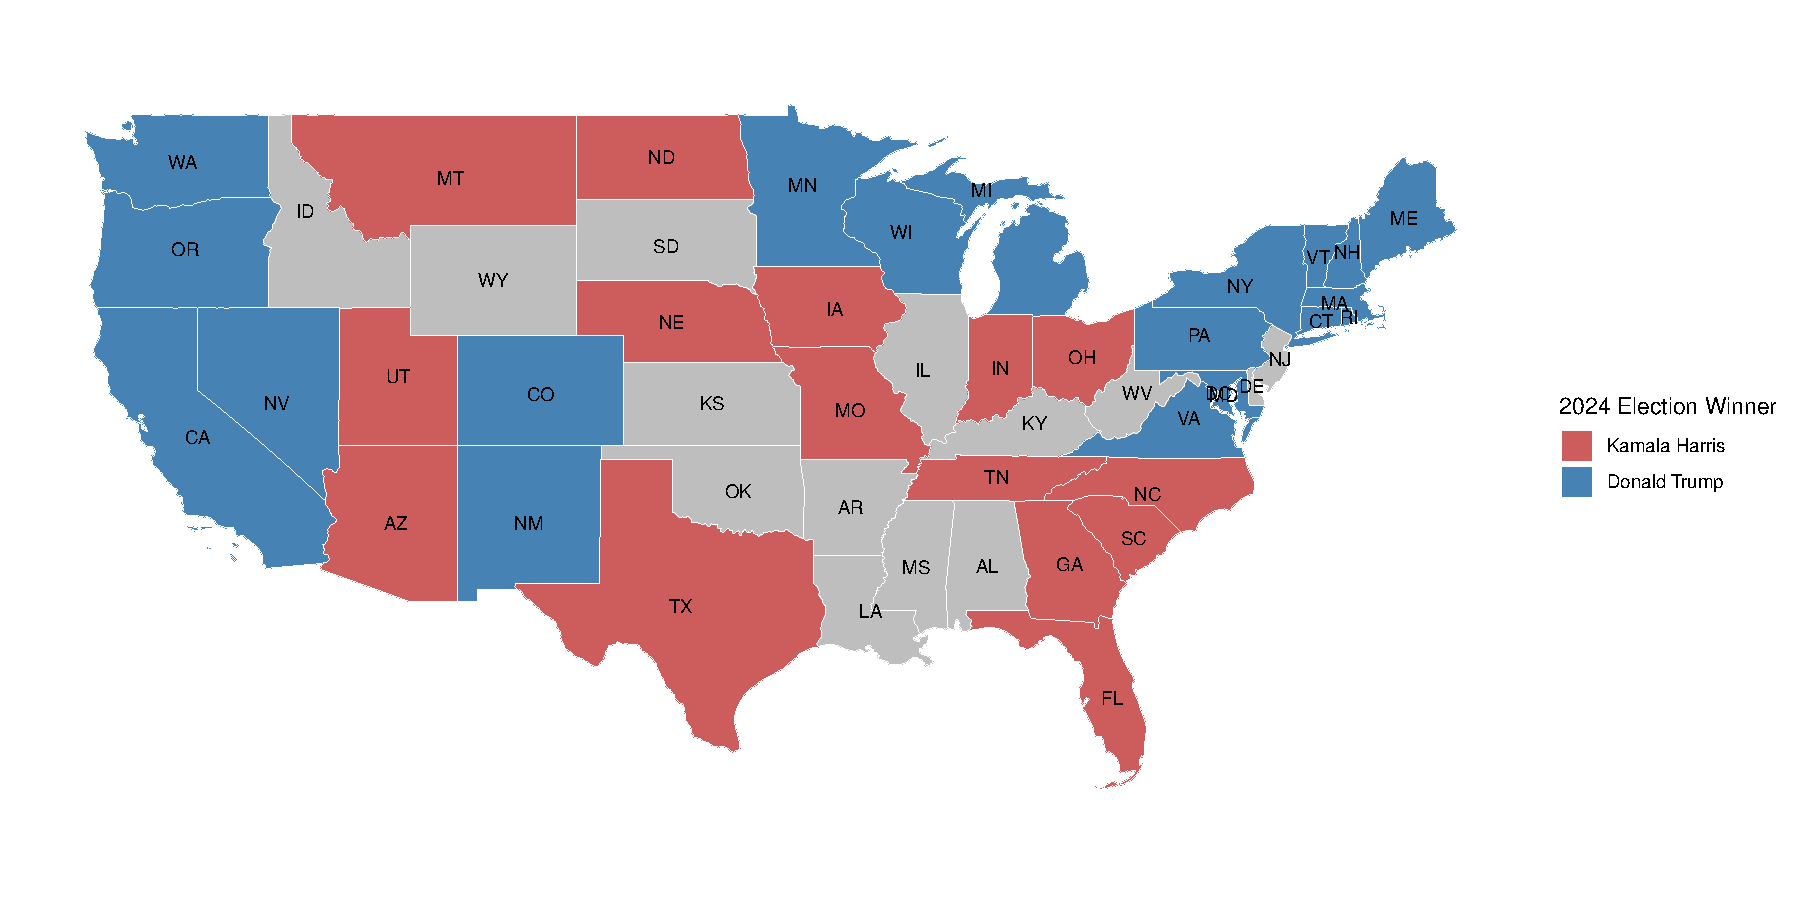
\includegraphics{paper_files/figure-pdf/fig-map2-1.pdf}

}

\caption{\label{fig-map2}Predicted 2024 U.S. Presidential Election
winner by state, with Kamala Harris-leaning states in blue, Donald
Trump-leaning states in red, and states lacking sufficient polling data
in gray. The map highlights traditional Democratic and Republican
strongholds as well as key battleground states.}

\end{figure}

Figure~\ref{fig-map2} presents the predicted winner of the 2024 U.S.
Presidential Election by state based on aggregated polling data, with
red representing states projected to favor Kamala Harris and blue
indicating those favoring Donald Trump. Notably, traditional Democratic
strongholds in the Northeast and West Coast, such as California, New
York, and Washington, show solid support for Harris. Conversely,
traditional Republican states, including Texas, Florida, and much of the
South, show strong support for Trump.

Swing states, like Pennsylvania, Michigan, and Wisconsin, are
predominantly leaning toward Harris, indicating a possible advantage for
her in these key battlegrounds, although other typical swing states like
Arizona and Georgia lean toward Trump. Gray-shaded states lack
sufficient polling data to make a prediction, reflecting areas of data
scarcity in the model's projections. This visualization highlights the
geographical and political divides across the U.S., as well as the
critical role swing states play in determining the election outcome.

\hypertarget{tbl-battleground-states}{}
\begin{longtable}[]{@{}
  >{\raggedright\arraybackslash}p{(\columnwidth - 8\tabcolsep) * \real{0.1705}}
  >{\raggedleft\arraybackslash}p{(\columnwidth - 8\tabcolsep) * \real{0.2159}}
  >{\raggedleft\arraybackslash}p{(\columnwidth - 8\tabcolsep) * \real{0.2045}}
  >{\raggedright\arraybackslash}p{(\columnwidth - 8\tabcolsep) * \real{0.1932}}
  >{\raggedleft\arraybackslash}p{(\columnwidth - 8\tabcolsep) * \real{0.2159}}@{}}
\caption{\label{tbl-battleground-states}Predicted support for Kamala
Harris and Donald Trump across key battleground states, indicating the
winner and the support margin (\%) in each state.}\tabularnewline
\toprule\noalign{}
\begin{minipage}[b]{\linewidth}\raggedright
State
\end{minipage} & \begin{minipage}[b]{\linewidth}\raggedleft
Kamala Support (\%)
\end{minipage} & \begin{minipage}[b]{\linewidth}\raggedleft
Trump Support (\%)
\end{minipage} & \begin{minipage}[b]{\linewidth}\raggedright
Predicted Winner
\end{minipage} & \begin{minipage}[b]{\linewidth}\raggedleft
Support Margin (\%)
\end{minipage} \\
\midrule\noalign{}
\endfirsthead
\toprule\noalign{}
\begin{minipage}[b]{\linewidth}\raggedright
State
\end{minipage} & \begin{minipage}[b]{\linewidth}\raggedleft
Kamala Support (\%)
\end{minipage} & \begin{minipage}[b]{\linewidth}\raggedleft
Trump Support (\%)
\end{minipage} & \begin{minipage}[b]{\linewidth}\raggedright
Predicted Winner
\end{minipage} & \begin{minipage}[b]{\linewidth}\raggedleft
Support Margin (\%)
\end{minipage} \\
\midrule\noalign{}
\endhead
\bottomrule\noalign{}
\endlastfoot
Arizona & 46.89009 & 48.21778 & Donald Trump & 1.3276921 \\
Georgia & 47.09997 & 48.21968 & Donald Trump & 1.1197167 \\
Michigan & 47.44921 & 46.34289 & Kamala Harris & 1.1063207 \\
Nevada & 47.48644 & 46.47506 & Kamala Harris & 1.0113774 \\
North Carolina & 47.60615 & 47.87192 & Donald Trump & 0.2657668 \\
Pennsylvania & 48.01476 & 46.96981 & Kamala Harris & 1.0449520 \\
Wisconsin & 48.67186 & 46.50662 & Kamala Harris & 2.1652329 \\
\end{longtable}

USAFacts(USA Facts 2024),FiveThirtyEight(FiveThirtyEight 2024) and many
other polling websites are calling Arizona, Georgia, Michigan,
Pennsylvania, Wisconsin, North Carolina, Nevada the `swing states' of
the 2024 presidential election.Polling in swing states is crucial for
election predictions because these states, with their historically close
voting margins, often determine the overall outcome by tipping the
electoral balance toward one candidate.
Table~\ref{tbl-battleground-states} summarizes the predicted support
percentages for Kamala Harris and Donald Trump in key battleground
states, along with the predicted winner and the support margin. The data
shows close margins in these states, with some like Arizona and Georgia
leaning slightly towards Trump, while others such as Michigan and
Pennsylvania favor Harris by narrow margins. The support margin column
highlights the competitiveness of these states, with all margins below
2.2\%, indicating highly contested races.

\hypertarget{sec-discussion}{%
\section{Discussion}\label{sec-discussion}}

In this paper, we set out to predict the support for both Kamala Harris
and Donald Trump in the 2024 U.S. Presidential Election using a
``polls-of-polls'' approach. By aggregating multiple polls, we sought to
mitigate the inherent biases present in individual surveys, creating a
more accurate and balanced forecast across candidates. Our analysis was
driven by a linear regression model using key predictors, such as
pollster, sample size, state, and recency of the polls. After
calculating predicted values from the model, we applied a weighting
scheme based on each pollster's numeric grade and pollscore,
incorporating both reliability and bias. This weighted approach enabled
us to produce an overall prediction of candidate support, reflecting
variations across different states and polling organizations.

One key insight from our analysis is the importance of poll recency.
Including recency notably increased the model's explanatory power, with
improvements in R² and reductions in RMSE compared to models without it.
This underscores the dynamic nature of public opinion, where recent
events can influence voter perceptions and candidate support.

Our state-level analysis highlights close competition observed in key
battleground states, emphasizing their pivotal role in the 2024
election. Our model reveals that in states like Pennsylvania, Michigan,
and Wisconsin, support levels for Harris and Trump are nearly tied,
reflecting the intense contest for these critical electoral votes. The
predictions show that even minor shifts in support within these swing
states could decisively impact the overall election outcome. This
analysis shows the importance of regional polling in capturing nuanced
voter sentiment and the heightened influence that battleground states
hold in shaping the final results.

However, there are limitations to our approach. Our model assumes linear
relationships between predictors and candidate support, which might not
capture more complex or interaction-based trends. Additionally, while we
weighted polls based on their numeric grades, these scores may not fully
reflect each pollster's accuracy, leaving room for improvement. Future
research could explore non-linear methods, such as machine learning, to
capture potential interactions between variables. Refining the weighting
mechanism by considering pollster performance history or state-specific
polling nuances could further enhance predictive accuracy.

In conclusion, this paper contributes to election forecasting by
providing a comprehensive, weighted estimate of candidate support across
both national and state levels. While our predictions provide valuable
insights into potential election outcomes, the evolving nature of voter
sentiment and poll accuracy reflects the need for adaptive models that
account for ongoing changes in public opinion.

\newpage

\appendix

\hypertarget{appendix}{%
\section*{Appendix}\label{appendix}}
\addcontentsline{toc}{section}{Appendix}

\hypertarget{emerson-college-polling-methodology-october-14-16-2024}{%
\section{Emerson College Polling Methodology (October 14-16,
2024)}\label{emerson-college-polling-methodology-october-14-16-2024}}

\hypertarget{overview}{%
\subsection{Overview}\label{overview}}

Emerson College Polling, also known as ECP, is a nationally-ranked
polling center that aims to accurately reflect public opinion through a
mixed-mode methodology (Emerson College Polling 2024a). ECP conducted a
survey from October 14 to 16, 2024, targeting 1,000 likely voters in the
2024 U.S. Presidential Election. The poll measured voter preferences
between Kamala Harris and Donald Trump, revealing a near tie with Harris
at 50\% and Trump at 49\% (Emerson College Polling 2024b). Appendix A
takes a closer look at the methodology used by ECP for this poll.

\hypertarget{population-frame-and-sample-of-the-poll}{%
\subsection{Population, Frame, and Sample of the
Poll}\label{population-frame-and-sample-of-the-poll}}

To conduct a poll, it is important to first define the target
population, the sampling frame and the sample. Defining these elements
sets a clear direction for the research and assures a clear object of
research (Akman 2023).

The target population is the whole group of interest the researchers
would like to make conclusions on (University of Massachusetts 2022).
For the poll conducted by ECP in October, the target population is
likely voters in the U.S. elections (Emerson College Polling 2024b).
Choosing likely voters as the target population makes the poll results
more accurate as not all registered voters end up voting in the
Presidential Election. In fact, the last U.S. Presidential Election in
2020 only had 66.8\% of registered voters participate in the elections,
which is the highest voter turnout in the 21st century (U.S. Census
Bureau 2021). In ECP's methodology, likely voters are determined by a
combination of voter history, registration status, and demographic data.
These factors are self-reported (Emerson College Polling 2024b).

The sampling frame is the part inside of the target population that has
a chance to be sampled upon (University of Massachusetts 2022). In ECP's
methodology, the sampling frame is the voters that are on Aristotle's
database and on the online panel provided by CINT (Emerson College
Polling 2024a). Aristotle is an online source of voter and consumer data
that has serviced many large political campaigns, PACs and corporations
both within the U.S and abroad (Aristotle 2024). CINT is the largest
global research marketplace that connects researchers, such as Emerson,
to survey respondents (CINT 2024).

The sample of a study is the part of the sampling frame that is measured
and is part of the data set (University of Massachusetts 2022). In the
case of a poll like ECP's, the sample is the respondents of the survey.
These respondents are directly represented in the data set (Emerson
College Polling 2024b). The sample size is 1,000 likely voters chosen
arbitrarily from the sampling frame.

\hypertarget{sample-recruitment-and-approach}{%
\subsection{Sample Recruitment and
Approach}\label{sample-recruitment-and-approach}}

Emerson College used a mixed-mode sampling approach for its polling
(Emerson College Polling 2024a). Specifically, three primary modes were
used to collect data for its October 14-16, 2024 poll (Emerson College
Polling 2024b) :

\begin{itemize}
\item
  MMS-to-web text surveys: Respondents were contacted via text messages
  sent to cell phones. These messages directed participants to complete
  the survey online. This method was conducted using voter lists
  provided by Aristotle.
\item
  Interactive Voice Response (IVR): Landlines were targeted using
  automated phone calls where respondents could answer questions using
  their keypads. The contact information for this was also sourced from
  Aristotle's voter lists.
\item
  Online Panel from CINT: Emerson utilized a pre-screened, opt-in online
  panel of voters provided by CINT.
\end{itemize}

\hypertarget{advantages-and-trade-offs-in-mixed-mode-sampling}{%
\subsection{Advantages and Trade-offs in Mixed-Mode
Sampling}\label{advantages-and-trade-offs-in-mixed-mode-sampling}}

The multi-mode sampling approach used by ECP in this poll has many
advantages. By using multiple data collection methods, ECP reduces
coverage bias (Mora 2011). In a survey, coverage bias means there is
some part of the target population that has zero chance of being part of
the sample and will not be represented in the data (Cummins 2021). For
example, MMS-to-web surveys tend to attract responses from younger
voters and individuals who rely primarily on mobile devices, capturing a
segment that may otherwise be underrepresented. Interactive voice
response (IVR) calls target older and rural voters, who are more
inclined to use landlines. Online panels gather responses from
tech-savvy individuals who prefer online engagement over other methods.
Multi-mode sampling is also more cost-effective (Mora 2011). Automated
technologies such as MMS-to-text web surveys and IVR reduce expenses
compared to traditional live interviews. Lower costs allow the poll to
reach a larger sample size, which also results in more accurate and
representative conclusions (Charlesworth Author Services 2022). However,
using a multi-mode sampling approach also introduces a trade-off. This
sampling approach introduces a measurement error (Mora 2011). Each
method---whether IVR, web surveys, or online panels---brings its own
unique biases. Combining these creates inconsistencies between
respondent groups. This increases the overall margin of error by adding
variability.

\hypertarget{non-response-handling}{%
\subsection{Non-response Handling}\label{non-response-handling}}

ECP addresses non-response using a weighting system. The data is
adjusted based on demographic variables like age, gender, race,
education, and party affiliation, making the sample more representative
of the electorate (Emerson College Polling 2024a). Weights are applied
to even out under- and over-represented groups, making the data more
similar to the electorate (Elliott 2020).

\hypertarget{questionnaire-design}{%
\subsection{Questionnaire Design}\label{questionnaire-design}}

The Emerson survey is designed with simplicity and efficiency. One of
its strengths is its straightforward format, using clear and unambiguous
questions. This simplicity makes the survey easy for respondents to
understand. Another strength is its topical relevance. By focusing on
vote preferences and demographic splits, the survey provides timely
insights, especially valuable during election cycles. However, the
survey has some limitations. One is its lack of nuance; while it
captures basic voter preferences, it doesn't explore the motivations or
factors driving those choices in depth. Additionally, the various survey
modes can affect respondent engagement with the questions, which may
also influence the accuracy and depth of their answers.

\hypertarget{conclusion}{%
\subsection{Conclusion}\label{conclusion}}

Emerson College Polling's mixed-mode methodology is effective in
balancing cost with broad demographic reach. Its weighting techniques
contribute to reliable and accurate results despite non-responses. While
the use of multiple survey modes reduces coverage bias, other possible
biases---such as lack of nuance and combined measurement errors must be
considered during the analysis.

\hypertarget{idealized-methodology}{%
\section{Idealized Methodology}\label{idealized-methodology}}

\hypertarget{overview-1}{%
\subsection{Overview}\label{overview-1}}

This methodology outlines an election forecasting plan with a budget of
\$100,000. This survey is heavily inspired by TIPP Insights and Emerson
College Polling (ECP), which are two respected polling institutions.
TIPP Insights is known for accurately predicting major U.S. elections,
including presidential races, by combining traditional live phone
interviews with probability-based sampling (Rakich 2023). Their history
of reliable forecasts has made TIPP a trusted name in polling, that
specializes in capturing voter sentiment and representing diverse
demographics. Similarly, Emerson College is known for its mixed-mode
polling strategy, which combines Interactive Voice Response (IVR) with
online polling to reach both older, landline users and younger,
mobile-first voters (Emerson College Polling 2024a).

By incorporating techniques from both of these institutions, our
methodology aims to achieve high accuracy and broad demographic reach,
ensuring a balanced, cost-effective approach to election forecasting.

\hypertarget{sampling-approach}{%
\subsection{Sampling Approach}\label{sampling-approach}}

This idealized methodology employs a multi-mode hybrid sampling
approach, utilizing both probability-based and non-probability-based
methods. Combining both methods provides both accuracy and inclusivity
in polling. Overall, this method creates a more complete view of voter
preferences (Baker et al. 2013).

Probability-based methods include live phone interviews (landline and
cell), as used by TIPP. Live interviews are a direct, personal method of
collecting responses, with voter lists sourced from Aristotle (TIPP
Staff 2023). This method is effective in reaching older voters and
voters with less internet connectivity. Interactive Voice Response (IVR)
is also used, following Emerson's strategy for landline users (Emerson
College Polling 2024a), to balance costs and ensure representation of
less tech-savvy populations.

For non-probability methods, this approach includes MMS-to-web surveys
for mobile users, inspired by Emerson's MMS-to-web strategy (Emerson
College Polling 2024a). Likely voters receive multimedia messages on
their cell phones encouraging them to complete an online survey, which
helps reach younger, mobile-first voters. Additionally, online panel
recruitment is done through CINT. This follows TIPP's online panel
strategy, where a part of the survey is delivered to a pre-screened
panel (TIPP Staff 2023).

The combination of these sampling methods and collection methods ensures
a more accurate representation of voter groups, including
harder-to-reach populations.

\hypertarget{recruitment-strategy}{%
\subsection{Recruitment Strategy}\label{recruitment-strategy}}

By using Aristotle's voter lists and CINT's platform as a sampling
frame, the sample consists of likely voters. Likely voters are
determined based on registration status and past voting behavior
(Emerson College Polling 2024b). Quota sampling would be used to match
the demographic profile of the U.S. electorate. Quota sampling is a
sampling method that relies on a non-random selection of units based on
predetermined proportions (Nikolopoulou 2022). This ensures that
respondents in the sample reflect demographic variables such as age,
gender, race, and education level.

We would oversample key swing states like Pennsylvania, Arizona, and
Georgia (FitzGerald 2024). Key swing states are states where there is no
overwhelming support for a particular candidate or political party
(Barket 2020). The outcome in these states often determine the overall
result of the election, making them critical in securing a win in the
Electoral College. Oversampling these states allows a more accurate
forecasting in these battlegrounds, which are critical for predicting
the Electoral College outcome.

\hypertarget{data-validation}{%
\subsection{Data Validation}\label{data-validation}}

Given that the data is collected in a hybrid format, we would use
duplicate detection methods via IP addresses or phone numbers to
eliminate multiple responses from the same individual. Also, we would
implement attention checks to identify respondents who are not fully
engaged. Both duplicate respondents and unengaged respondents bias
results, and should be removed from the data set.

The data will be weighted to ensure that the sample aligns with key
demographics (race, gender, education) based on census data. Weights are
applied to even out under- and over-represented groups, making the data
more similar to the electorate (Elliott 2020).

\hypertarget{conclusion-1}{%
\subsection{Conclusion}\label{conclusion-1}}

By combining TIPP's live phone/IVR hybrid and Emerson College's
mixed-mode survey methods, this idealized methodology captures diverse
voter demographics. It uses both probability-based and
non-probability-based sampling methods to forecast the 2024 U.S.
Presidential Election.

A link to the survey can be found at:
https://forms.gle/haGLaQBPQhrXE6Xa7

\hypertarget{copy-of-the-survey}{%
\section{Copy of the Survey}\label{copy-of-the-survey}}

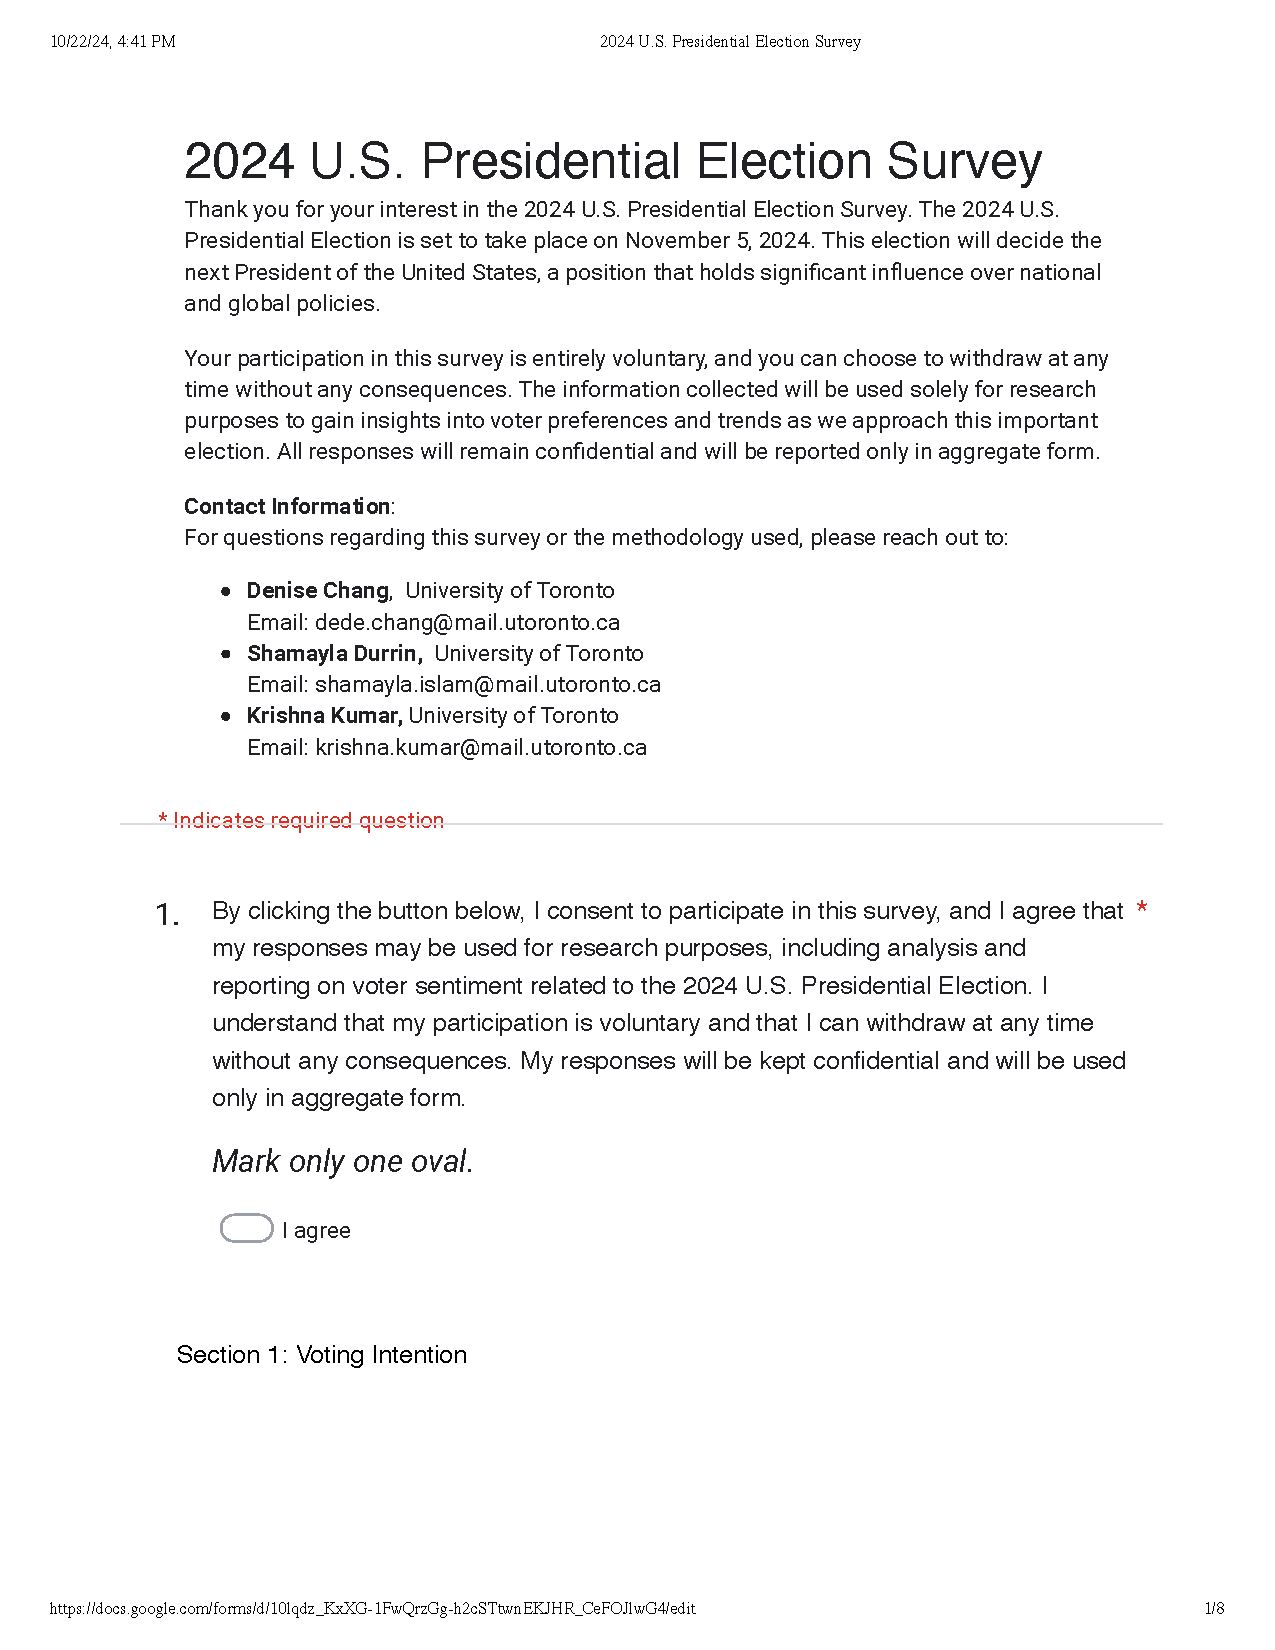
\includepdf[pages=-]{../other/surveyfiles/SurveyCopy.pdf}

\hypertarget{model-diagnostics}{%
\section{Model Diagnostics}\label{model-diagnostics}}

\begin{figure}

{\centering 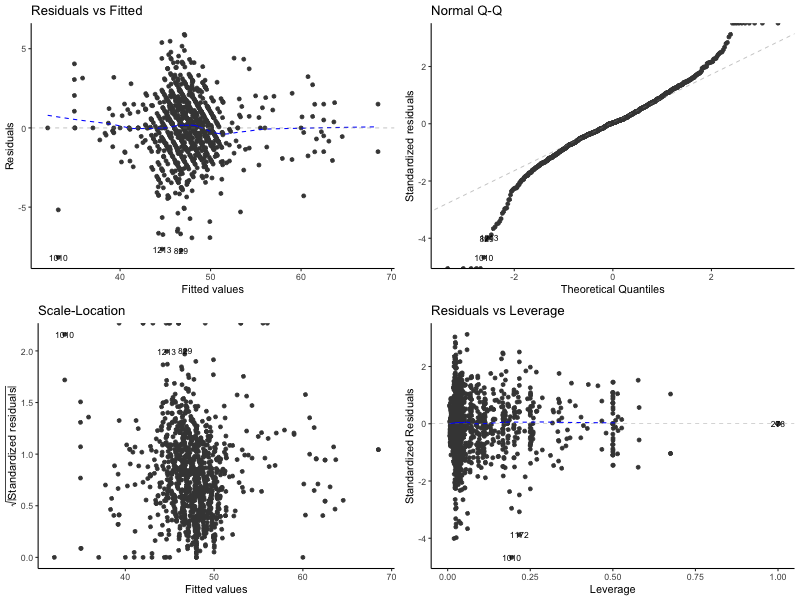
\includegraphics{../other/graphs/diagnostic_plot_model3.png}

}

\caption{\label{fig-dgplotone}\textbf{?(caption)}}

\end{figure}

The diagnostic plots for Model 3ni sgiven in Figure~\ref{fig-dgplotone}.
We notice the following:

\begin{enumerate}
\def\labelenumi{\arabic{enumi}.}
\item
  \textbf{Residuals vs.~Fitted Plot}: This plot checks for non-linearity
  and heteroscedasticity. The residuals are scattered around the
  horizontal axis with no clear pattern, indicating that the linearity
  assumption is reasonable. However, there is slight spread around the
  center, suggesting some mild heteroscedasticity.
\item
  \textbf{Normal Q-Q Plot}: This plot assesses the normality of
  residuals. Most points align along the diagonal line, although there
  are some deviations at the tails. This suggests that the residuals are
  approximately normally distributed, with minor deviations in the
  extremes.
\item
  \textbf{Scale-Location Plot}: This plot further checks for
  homoscedasticity. The residuals appear to be evenly spread across the
  fitted values, supporting the homoscedasticity assumption, although
  slight deviations are present in certain regions.
\item
  \textbf{Residuals vs.~Leverage Plot}: This plot identifies potential
  influential points. While most points have low leverage, a few points
  exhibit higher leverage, as indicated by their distance from the
  center. However, no points exceed Cook's distance threshold,
  indicating no extreme outliers that would unduly influence the model.
\end{enumerate}

\begin{figure}

{\centering 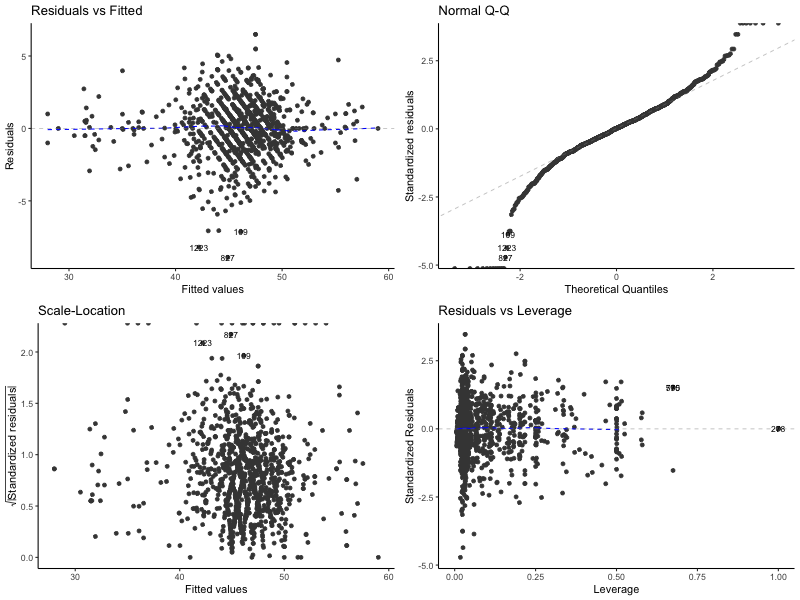
\includegraphics{../other/graphs/diagnostic_plot_model6.png}

}

\caption{\label{fig-dgplottwo}\textbf{?(caption)}}

\end{figure}

The diagnostic plots for Model 6 is given in Figure~\ref{fig-dgplottwo}.
We notice the following:

\begin{enumerate}
\def\labelenumi{\arabic{enumi}.}
\item
  \textbf{Residuals vs Fitted}: This plot suggests a fairly random
  spread of residuals around zero, indicating that the linearity
  assumption holds reasonably well. However, there is slight clustering
  of points in the center, which could indicate minor heteroscedasticity
  but is not severe.
\item
  \textbf{Normal Q-Q Plot}: The Q-Q plot shows that the residuals
  generally follow a normal distribution, with only a few deviations at
  the tails. This suggests that the normality assumption is mostly met,
  though some minor deviations in the upper tail indicate possible
  outliers.
\item
  \textbf{Scale-Location (Spread-Location) Plot}: The residuals appear
  randomly dispersed with no clear pattern, supporting the
  homoscedasticity (constant variance) assumption. However, some
  observations near the upper range might indicate slight variance
  inconsistency, though it is minimal.
\item
  \textbf{Residuals vs Leverage}: This plot does not show any
  influential outliers with high leverage that might impact the model
  unduly. The Cook's distance lines show that no data points exceed
  these thresholds, indicating that no individual observation is
  disproportionately influencing the model.
\end{enumerate}

Overall, the diagnostic plots for both model suggests that they meet the
assumptions for linear regression fairly well, with minor deviations
that are not expected to severely impact the model's validity.

\hypertarget{code-styling}{%
\section{Code Styling}\label{code-styling}}

The code in this paper was reviewed and formatted for consistency using
lintr (Hester et al. 2024) and styler (Müller and Walthert 2024),
ensuring readability and adherence to style standards.

\hypertarget{reproducibility}{%
\section{Reproducibility}\label{reproducibility}}

To replicate the findings presented in this paper, users should execute
the scripts available in the GitHub repository. Begin by running the
00-install\_packages.R script, which installs all required packages for
the analysis.

\hypertarget{acknowledgments}{%
\section{Acknowledgments}\label{acknowledgments}}

We extend our gratitude to (Alexander 2023), which provided invaluable
guidance in establishing a reproducible workflow and inspired many of
the code structures used in this paper.

\newpage

\hypertarget{references}{%
\section*{References}\label{references}}
\addcontentsline{toc}{section}{References}

\hypertarget{refs}{}
\begin{CSLReferences}{1}{0}
\leavevmode\vadjust pre{\hypertarget{ref-def_pred_bias}{}}%
Aguinis, Herman, and Steven Culpepper. 2024. \emph{Improving Our
Understanding of Predictive Bias in Testing}.
\url{https://psycnet.apa.org/fulltext/2024-15734-001.html}.

\leavevmode\vadjust pre{\hypertarget{ref-akman}{}}%
Akman, Sena. 2023. \emph{What Is Target Population: Definition \&
Examples}. \url{https://forms.app/en/blog/target-population}.

\leavevmode\vadjust pre{\hypertarget{ref-citeTS}{}}%
Alexander, Rohan. 2023. {``Telling Stories with Data.''} Chapman;
Hall/CRC. \url{https://tellingstorieswithdata.com/}.

\leavevmode\vadjust pre{\hypertarget{ref-aristotle}{}}%
Aristotle. 2024. \emph{Data}. \url{https://www.aristotle.com/data/}.

\leavevmode\vadjust pre{\hypertarget{ref-baker}{}}%
Baker, Reg, Michael Brick, Nancy Bates, Mike Battaglia, Mick Couper,
Jill Dever, Krista Gile, and Roger Tourangeau. 2013. \emph{REPORT OF THE
AAPOR TASK FORCE ON NONPROBABILITY SAMPLING}.
\url{https://aapor.org/wp-content/uploads/2022/11/NPS_TF_Report_Final_7_revised_FNL_6_22_13-2.pdf}.

\leavevmode\vadjust pre{\hypertarget{ref-barker}{}}%
Barket, Elaine. 2020. \emph{Recommendation for Key Management: Part 1 --
General}.
\url{https://nvlpubs.nist.gov/nistpubs/SpecialPublications/NIST.SP.800-57pt1r5.pdf}.

\leavevmode\vadjust pre{\hypertarget{ref-large_ss}{}}%
Charlesworth Author Services. 2022. \emph{The Importance of Having Large
Sample Sizes for Your Research}.
\url{https://www.cwauthors.com/article/importance-of-having-large-sample-sizes-for-research}.

\leavevmode\vadjust pre{\hypertarget{ref-cint}{}}%
CINT. 2024. \emph{Cint}. \url{https://www.cint.com/}.

\leavevmode\vadjust pre{\hypertarget{ref-def_cb}{}}%
Cummins, Emily. 2021. \emph{Coverage Bias: Definition \& Examples}.
\url{https://study.com/academy/lesson/coverage-bias-definition-examples.html}.

\leavevmode\vadjust pre{\hypertarget{ref-weight}{}}%
Elliott, Roxana. 2020. \emph{Weighting Survey Data: Methods and
Advantages}.
\url{https://www.geopoll.com/blog/weighting-survey-data-raking-cell-weighting/}.

\leavevmode\vadjust pre{\hypertarget{ref-about_ecp}{}}%
Emerson College Polling. 2024a. \emph{About Us}.
\url{https://emersoncollegepolling.com/about/}.

\leavevmode\vadjust pre{\hypertarget{ref-ecp_poll}{}}%
---------. 2024b. \emph{October 2024 Tracking National Poll: Harris 49}.
\url{https://emersoncollegepolling.com/october-2024-tracking-national-poll-harris-49-trump-48/}.

\leavevmode\vadjust pre{\hypertarget{ref-janitor}{}}%
Firke, Sam. 2023. \emph{Janitor: Simple Tools for Examining and Cleaning
Dirty Data}. \url{https://CRAN.R-project.org/package=janitor}.

\leavevmode\vadjust pre{\hypertarget{ref-swing_state}{}}%
FitzGerald, James. 2024. \emph{The Seven Swing States Set to Decide the
2024 US Election}. \url{https://www.bbc.com/news/articles/c511pyn3xw3o}.

\leavevmode\vadjust pre{\hypertarget{ref-FiveThirtyEight}{}}%
FiveThirtyEight. 2024. {``{FiveThirtyEight U.S. Election Polls}.''}
\url{https://projects.fivethirtyeight.com/polls/}.

\leavevmode\vadjust pre{\hypertarget{ref-citelintr}{}}%
Hester, Jim, Florent Angly, Russ Hyde, Michael Chirico, Kun Ren,
Alexander Rosenstock, and Indrajeet Patil. 2024. \emph{Lintr: A 'Linter'
for r Code}. \url{https://CRAN.R-project.org/package=lintr}.

\leavevmode\vadjust pre{\hypertarget{ref-mora}{}}%
Mora, Michaela. 2011. \emph{Understanding the Pros and Cons of
Mixed-Mode Research}.
\url{https://www.relevantinsights.com/articles/pros-and-cons-of-mixed-mode-research/}.

\leavevmode\vadjust pre{\hypertarget{ref-538_morris}{}}%
Morris, Elliott. 2024a. \emph{How 538's Pollster Ratings Work}.
\url{https://abcnews.go.com/538/538s-pollster-ratings-work/story?id=105398138}.

\leavevmode\vadjust pre{\hypertarget{ref-538_methodology}{}}%
---------. 2024b. \emph{Trump Leads in Swing-State Polls and Is Tied
with Biden Nationally}.
\url{https://abcnews.go.com/538/trump-leads-swing-state-polls-tied-biden-nationally/story?id=109506070}.

\leavevmode\vadjust pre{\hypertarget{ref-citestyler}{}}%
Müller, Kirill, and Lorenz Walthert. 2024. \emph{Styler: Non-Invasive
Pretty Printing of r Code}.
\url{https://CRAN.R-project.org/package=styler}.

\leavevmode\vadjust pre{\hypertarget{ref-def_quota}{}}%
Nikolopoulou, Kassiani. 2022. \emph{What Is Quota Sampling? \textbar{}
Definition \& Examples}.
\url{https://www.scribbr.com/methodology/quota-sampling/}.

\leavevmode\vadjust pre{\hypertarget{ref-citeR}{}}%
R Core Team. 2024. \emph{R: A Language and Environment for Statistical
Computing}. Vienna, Austria: R Foundation for Statistical Computing.
\url{https://www.R-project.org/}.

\leavevmode\vadjust pre{\hypertarget{ref-tipp_accuracy}{}}%
Rakich, Nathaniel. 2023. \emph{The Polls Were Historically Accurate in
2022}.
\url{https://fivethirtyeight.com/features/2022-election-polling-accuracy/}.

\leavevmode\vadjust pre{\hypertarget{ref-def_pred_error}{}}%
Renewable Energy. 2012. \emph{Prediction Error}.
\url{https://www.sciencedirect.com/topics/engineering/prediction-error}.

\leavevmode\vadjust pre{\hypertarget{ref-arrow}{}}%
Richardson, Neal, Ian Cook, Nic Crane, Dewey Dunnington, Romain
François, Jonathan Keane, Dragoș Moldovan-Grünfeld, Jeroen Ooms, Jacob
Wujciak-Jens, and Apache Arrow. 2024. \emph{Arrow: Integration to
'Apache' 'Arrow'}. \url{https://CRAN.R-project.org/package=arrow}.

\leavevmode\vadjust pre{\hypertarget{ref-tipp_methodology}{}}%
TIPP Staff. 2023. \emph{TIPP Indexes Methodology}.
\url{https://tippinsights.com/tipp-indexes-methodology/}.

\leavevmode\vadjust pre{\hypertarget{ref-def_terms}{}}%
University of Massachusetts. 2022. \emph{Populations and Samples}.
\url{https://people.umass.edu/~biep540w/pdf/sampling.pdf}.

\leavevmode\vadjust pre{\hypertarget{ref-us_census}{}}%
U.S. Census Bureau. 2021. \emph{2020 Presidential Election Voting and
Registration Tables Now Available}.
\url{https://www.census.gov/newsroom/press-releases/2021/2020-presidential-election-voting-and-registration-tables-now-available.html}.

\leavevmode\vadjust pre{\hypertarget{ref-usafacts}{}}%
USA Facts. 2024. {``{What Are the Current Swing States and How Have They
Changed Over Time?}''}
\url{https://usafacts.org/articles/what-are-the-current-swing-states-and-how-have-they-changed-over-time/}.

\leavevmode\vadjust pre{\hypertarget{ref-tidy}{}}%
Wickham, Hadley, Mara Averick, Jennifer Bryan, Winston Chang, Lucy
D'Agostino McGowan, Romain François, Garrett Grolemund, et al. 2019.
{``Welcome to the {tidyverse}.''} \emph{Journal of Open Source Software}
4 (43): 1686. \url{https://doi.org/10.21105/joss.01686}.

\end{CSLReferences}



\end{document}
